\documentclass[11pt,a4paper]{article}

\usepackage[utf8]{inputenc}
\usepackage[
  left=1.05in,
  right=1.05in,
  top=1in,
  bottom=1in,
  headheight=14pt
]{geometry}
\usepackage{amsmath,amssymb,amsthm,mathtools}
\usepackage{bm}
\usepackage{enumitem}
\usepackage{booktabs,array}
\usepackage{microtype}
\usepackage[dvipsnames]{xcolor}
\usepackage{tikz}
\usepackage[breakable,skins]{tcolorbox}
\usepackage[hidelinks]{hyperref}
\usepackage{fancyhdr}

\linespread{1.25}
\setlength{\parindent}{0pt}
\setlength{\parskip}{1em plus 0.25em minus 0.1em}
\setlength{\abovedisplayskip}{1.3em plus 0.3em minus 0.2em}
\setlength{\belowdisplayskip}{1.3em plus 0.3em minus 0.2em}
\setlength{\abovedisplayshortskip}{1em plus 0.2em}
\setlength{\belowdisplayshortskip}{1.1em plus 0.2em}
\setlength{\jot}{10pt}
\setlength{\emergencystretch}{2em}
\raggedbottom

\numberwithin{equation}{section}

\newtheoremstyle{spacedplain}
  {18pt}{18pt}{\itshape}{}{\bfseries}{.}{0.5em}{}
\newtheoremstyle{spaceddefinition}
  {18pt}{18pt}{\normalfont}{}{\bfseries}{.}{0.5em}{}
\newtheoremstyle{spacedremark}
  {18pt}{18pt}{\normalfont}{}{\itshape}{.}{0.5em}{}

\theoremstyle{spacedplain}
\newtheorem{theorem}{Theorem}[section]
\newtheorem{lemma}[theorem]{Lemma}
\newtheorem{proposition}[theorem]{Proposition}
\newtheorem{corollary}[theorem]{Corollary}

\theoremstyle{spaceddefinition}
\newtheorem{definition}[theorem]{Definition}
\newtheorem{example}[theorem]{Example}
\newtheorem{exercise}[theorem]{Exercise}

\theoremstyle{spacedremark}
\newtheorem{remark}[theorem]{Remark}

\setlist[itemize]{leftmargin=*,itemsep=7pt,topsep=8pt,parsep=3pt}
\setlist[enumerate]{leftmargin=*,itemsep=7pt,topsep=8pt,parsep=3pt}

% Plain black frame, used only for the most important results.
\newtcolorbox{keybox}{
  enhanced,
  colback=white,colframe=black,
  boxrule=0.6pt,sharp corners,
  left=10pt,right=10pt,top=4pt,bottom=6pt,
  before skip=16pt,after skip=16pt
}

\pagestyle{fancy}
\fancyhf{}
\fancyhead[L]{MTL712}
\fancyhead[R]{Numerical Methods for ODEs and PDEs}
\fancyfoot[C]{\thepage}
\renewcommand{\headrulewidth}{0.4pt}
\renewcommand{\footrulewidth}{0pt}

% Run-in headings inside proofs and sections, set on their own line.
\newcommand{\step}[1]{\par\addvspace{0.6em}\noindent\textbf{#1}\par\nobreak}

\newcommand{\pd}[2]{\frac{\partial #1}{\partial #2}}
\newcommand{\pdd}[2]{\frac{\partial^2 #1}{\partial #2^2}}
\newcommand{\hb}{\bar h}

\title{\textbf{MTL712: Computational Methods for Differential\\Equations}\\[6pt]
\large Multistep Methods, Boundary Value Problems, and\\
Finite Differences for Parabolic PDEs}
\author{\normalsize Typeset lecture notes}
\date{}

\begin{document}

\maketitle
\thispagestyle{plain}
{\linespread{1.0}\selectfont\setlength{\parskip}{0pt}\tableofcontents}
\clearpage

%#####################################################################
\part{Linear Multistep Methods for \(y'=f(x,y)\)}
%#####################################################################

\section{The Setting}

We solve the initial value problem
\[
  y'=f(x,y),\qquad y(x_0)=y_0,
\]
on the grid \(x_n=x_0+nh\).

\begin{definition}[Linear multistep method]
A \emph{linear \(k\)-step method} (LMM) is
\begin{equation}\label{eq:lmm}
  \sum_{j=0}^k\alpha_j\,y_{n+j}
  =h\sum_{j=0}^k\beta_j\,f_{n+j},
  \qquad f_{n+j}=f(x_{n+j},y_{n+j}),
\end{equation}
with
\[
  \alpha_k\ne0,\qquad |\alpha_0|+|\beta_0|>0.
\]
It is \emph{explicit} if \(\beta_k=0\) and \emph{implicit} if
\(\beta_k\neq 0\).
\end{definition}

\begin{definition}[Characteristic polynomials]
The first and second characteristic polynomials are
\[
\begin{gathered}
  \rho(\zeta)=\sum_{j=0}^k\alpha_j\zeta^j,
  \\
  \sigma(\zeta)=\sum_{j=0}^k\beta_j\zeta^j.
\end{gathered}
\]
With the shift operator \(Ey_n=y_{n+1}\), the method is simply
\[
  \rho(E)\,y_n=h\,\sigma(E)\,f_n.
\]
\end{definition}

\begin{definition}[Difference operator, order, error constant]
The linear difference operator associated with \eqref{eq:lmm} is
\[
  L[y(x);h]
  =\sum_{j=0}^k\bigl[\alpha_j\,y(x+jh)-h\,\beta_j\,y'(x+jh)\bigr].
\]
By Taylor expansion,
\[
  L[y(x);h]=C_0y(x)+C_1h\,y'(x)+C_2h^2y''(x)+\cdots,
\]
where
\[
\begin{gathered}
  C_0=\sum_{j}\alpha_j,
  \\
  C_1=\sum_{j} j\alpha_j-\sum_{j}\beta_j,
\end{gathered}
\]
and, for \(q\ge2\),
\[
  C_q=\frac1{q!}\sum_{j} j^q\alpha_j
      -\frac1{(q-1)!}\sum_{j} j^{q-1}\beta_j .
\]
The method has \emph{order \(p\)} if
\[
  C_0=C_1=\cdots=C_p=0,
  \qquad C_{p+1}\ne0.
\]
Then \(C_{p+1}\) is the \emph{error constant}, and the local
truncation error is
\[
  L[y(x_n);h]=C_{p+1}h^{p+1}y^{(p+1)}(x_n)+O(h^{p+2}).
\]
\end{definition}

\begin{definition}[Consistency and zero-stability]
\leavevmode
\begin{itemize}
  \item The method is \emph{consistent} if it has order \(p\ge1\),
    that is,
    \[
      C_0=C_1=0
      \iff
      \rho(1)=0\ \text{ and }\ \rho'(1)=\sigma(1).
    \]
  \item The method is \emph{zero-stable} (satisfies the \emph{root
    condition}) if every root of \(\rho\) satisfies
    \(|\zeta|\le1\), and every root with \(|\zeta|=1\) is simple.
\end{itemize}
\end{definition}

\begin{keybox}
\begin{lemma}[Order via \(\varphi\)]\label{lem:order}
Let
\[
  \varphi(\zeta)=\frac{\rho(\zeta)}{\log\zeta}-\sigma(\zeta).
\]
The LMM \eqref{eq:lmm} has order \(p\) if and only if \(\varphi\) has a
zero of exact multiplicity \(p\) at \(\zeta=1\).  In that case
\[
  \varphi(\zeta)=C_{p+1}(\zeta-1)^p+O\bigl((\zeta-1)^{p+1}\bigr).
\]
\end{lemma}
\end{keybox}

\begin{proof}\leavevmode
\step{Step 1: apply \(L\) to \(e^x\)}
Every derivative of \(e^x\)
equals \(1\) at \(x=0\).  Hence
\[
  g(h):=L[e^x;h]\big|_{x=0}
  =\sum_j\bigl(\alpha_je^{jh}-h\beta_je^{jh}\bigr)
  =\rho(e^h)-h\,\sigma(e^h)
  =\sum_{q\ge0}C_qh^q ,
\]
so \(C_q=g^{(q)}(0)/q!\).

\step{Step 2: change variable}
Put \(\zeta=e^h\), so
\(h=\log\zeta\), and \(\zeta\to1\iff h\to0\).  Then
\[
  g(\log\zeta)
  =\rho(\zeta)-\log\zeta\,\sigma(\zeta)
  =\log\zeta\cdot\varphi(\zeta).
\]

\step{Step 3 (\(\Leftarrow\))}
Suppose
\[
  \varphi(\zeta)=c(\zeta-1)^p+O\bigl((\zeta-1)^{p+1}\bigr),
  \qquad c\ne0.
\]
Since \(\zeta-1=e^h-1=h+O(h^2)\), we have
\((\zeta-1)^p=h^p+O(h^{p+1})\), so
\[
  g(h)=h\,\varphi(e^h)
  =h\bigl[c\,h^p+O(h^{p+1})\bigr]
  =c\,h^{p+1}+O(h^{p+2}).
\]
Comparing with \(g(h)=\sum C_qh^q\) gives
\(C_0=C_1=\cdots=C_p=0\) and \(C_{p+1}=c\ne0\).  Consequently the
method has order \(p\).

\step{Step 4 (\(\Rightarrow\))}
If the order is \(p\), then
\(g(h)=C_{p+1}h^{p+1}+O(h^{p+2})\), so
\[
  \varphi(\zeta)
  =\frac{g(\log\zeta)}{\log\zeta}
  =C_{p+1}(\log\zeta)^p+\cdots
  =C_{p+1}(\zeta-1)^p+O\bigl((\zeta-1)^{p+1}\bigr),
\]
using \(\log\zeta=(\zeta-1)+O\bigl((\zeta-1)^2\bigr)\).
\end{proof}

\section{Constructing Methods of Maximal Order (Henrici)}

\begin{keybox}
\begin{theorem}[Henrici]\label{thm:henrici}
Let \(\rho(\zeta)\) be a polynomial of degree \(k\) with
\[
  \rho(1)=0,\qquad \rho'(1)\ne0,
\]
and let \(k'\) be an integer with \(0\le k'\le k\).  Then there exists
a unique polynomial \(\sigma(\zeta)\) of degree \(\le k'\) such that
the linear \(k\)-step method associated with \(\rho\) and \(\sigma\)
has order \(\ge k'+1\).
\end{theorem}
\end{keybox}

Taking \(k'=k\) gives a method of order \(\ge k+1\), which is
\emph{implicit} unless the coefficient of \((\zeta-1)^k\) happens to
vanish; taking \(k'=k-1\) always gives an \emph{explicit} method of
order \(\ge k\).

\begin{proof}\leavevmode
\step{Step 1: \(\rho(\zeta)/\log\zeta\) has a Taylor series}
Both
\(\rho\) and \(\log\zeta\) have a simple zero at \(\zeta=1\), so the
zeros cancel and \(\rho(\zeta)/\log\zeta\) is holomorphic in a
neighbourhood of \(\zeta=1\).  It can therefore be expanded in a
convergent Taylor series
\[
  \frac{\rho(\zeta)}{\log\zeta}
  =c_0+c_1(\zeta-1)+c_2(\zeta-1)^2+\cdots.
\]

\step{Step 2: \(c_0=\rho'(1)\ne0\)}
Multiply by \(\log\zeta\):
\[
  \rho(\zeta)=\log\zeta\,\bigl[c_0+c_1(\zeta-1)+\cdots\bigr].
\]
Differentiating,
\[
  \rho'(\zeta)
  =\frac1\zeta\bigl[c_0+c_1(\zeta-1)+\cdots\bigr]
   +\log\zeta\,\bigl[c_1+2c_2(\zeta-1)+\cdots\bigr].
\]
At \(\zeta=1\), \(\log 1=0\), so \(\rho'(1)=c_0\).

\step{Step 3: define \(\sigma\)}
Let
\[
  \sigma(\zeta)=c_0+c_1(\zeta-1)+\cdots+c_{k'}(\zeta-1)^{k'}.
\]
Then \(\sigma(1)=c_0=\rho'(1)\ne0\), so the method is consistent.
With this definition,
\[
  \varphi(\zeta)
  =\frac{\rho(\zeta)}{\log\zeta}-\sigma(\zeta)
  =c_{k'+1}(\zeta-1)^{k'+1}+c_{k'+2}(\zeta-1)^{k'+2}+\cdots,
\]
so \(\varphi\) has a zero at \(\zeta=1\) of multiplicity at least
\(k'+1\).

\step{Step 4: order}
By Lemma~\ref{lem:order}, the method
associated with \(\rho\) and \(\sigma\) has order \(\ge k'+1\).

\step{Step 5: uniqueness}
Any \(\sigma\) of degree \(\le k'\)
giving order \(\ge k'+1\) must agree with \(\rho/\log\zeta\) up to the
\((\zeta-1)^{k'}\) term.  Uniqueness of \(\sigma\) therefore follows
from the uniqueness of the Taylor expansion of
\(\rho(\zeta)/\log\zeta\) at \(\zeta=1\).
\end{proof}

\begin{example}\label{ex:henrici}
Let \(\rho(\zeta)=(\zeta-1)(\zeta-\lambda)\), with \(\lambda\) real and
\(-1\le\lambda<1\).  Find \(\sigma\) giving the implicit method of
maximal order, and write the methods explicitly for \(\lambda=0\) and
\(\lambda=-1\).
\end{example}

\begin{proof}[Solution]
Here \(k=2\).  Implicit means \(k'=k=2\) (explicit would be
\(k'=k-1=1\)).  Write \(w=\zeta-1\), so
\[
  \rho=w\,\bigl[(1-\lambda)+w\bigr].
\]
Using
\[
\begin{gathered}
  \log(1+w)=w-\frac{w^2}{2}+\frac{w^3}{3}-\cdots,
  \\
  \frac{w}{\log(1+w)}=1+\frac w2-\frac{w^2}{12}+\frac{w^3}{24}-\cdots,
\end{gathered}
\]
we get
\begin{align*}
  \frac{\rho(\zeta)}{\log\zeta}
  &=\bigl[(1-\lambda)+w\bigr]
    \Bigl[1+\frac w2-\frac{w^2}{12}+\frac{w^3}{24}-\cdots\Bigr]\\
  &=(1-\lambda)+\frac{3-\lambda}{2}\,w+\frac{5+\lambda}{12}\,w^2
    -\frac{1+\lambda}{24}\,w^3+O(w^4).
\end{align*}
Keeping terms up to \(w^2\),
\begin{align*}
  \sigma(\zeta)
  &=(1-\lambda)+\frac{3-\lambda}2(\zeta-1)
    +\frac{5+\lambda}{12}(\zeta-1)^2\\
  &=-\frac{1+5\lambda}{12}+\frac{2(1-\lambda)}{3}\,\zeta
    +\frac{5+\lambda}{12}\,\zeta^2 .
\end{align*}
The method is
\[
  y_{n+2}-(1+\lambda)y_{n+1}+\lambda y_n
  =h\Bigl[\frac{5+\lambda}{12}f_{n+2}
         +\frac{2(1-\lambda)}3f_{n+1}
         -\frac{1+5\lambda}{12}f_n\Bigr].
\]
\begin{itemize}
  \item If \(\lambda\ne-1\), the order is \(3\) and the error constant
    is the first omitted coefficient,
    \[
      C_4=-\frac{1+\lambda}{24}.
    \]
  \item \(\lambda=0\): \(\rho(\zeta)=\zeta^2-\zeta\) and
    \(\sigma(\zeta)=\frac1{12}(5\zeta^2+8\zeta-1)\).  This is the
    \emph{Adams--Moulton} method
    \[
      y_{n+2}-y_{n+1}=\frac h{12}\bigl(5f_{n+2}+8f_{n+1}-f_n\bigr),
    \]
    or, shifted by one index,
    \(y_{n+1}-y_n=\frac h{12}\bigl(5f_{n+1}+8f_n-f_{n-1}\bigr)\).
  \item \(\lambda=-1\): the \(w^3\) coefficient vanishes, so the order
    is \(4\).  This is the \emph{Milne--Simpson} method
    \[
      y_{n+2}-y_n=\frac h3\bigl(f_{n+2}+4f_{n+1}+f_n\bigr),
      \qquad C_5=-\frac1{90}.
    \]
\end{itemize}
\end{proof}

\begin{remark}[Recipe]
\leavevmode
\begin{itemize}
  \item \emph{\(\rho\) given:} expand \(\rho(\zeta)/\log\zeta\) as a
    Taylor series in powers of \((\zeta-1)\).  Then
    \[
      \frac{\rho(\zeta)}{\log\zeta}-\sigma(\zeta)
      =C_{p+1}(\zeta-1)^p+O\bigl((\zeta-1)^{p+1}\bigr).
    \]
    Truncate after \((\zeta-1)^k\) (implicit) or \((\zeta-1)^{k-1}\)
    (explicit).
  \item \emph{\(\sigma\) given:} expand \((\log\zeta)\,\sigma(\zeta)\)
    in powers of \((\zeta-1)\) and truncate to obtain \(\rho\).
\end{itemize}
There is no consistent zero-stable \(k\)-step method of order
\(>k+2\); the next theorem gives this bound, and the sharper bound
\(k+1\) when \(k\) is odd.
\end{remark}

\section{The First Dahlquist Barrier}

\begin{keybox}
\begin{theorem}[First Dahlquist barrier]\label{thm:dahlquist}
There is no zero-stable linear \(k\)-step method whose order exceeds
\(k+1\) if \(k\) is odd, or \(k+2\) if \(k\) is even.
\end{theorem}
\end{keybox}

\begin{definition}[Optimal method]
A zero-stable linear \(k\)-step method of order \(k+2\) is called an
\emph{optimal method}.
\end{definition}

Optimal methods exist only for even \(k\); Milne--Simpson (\(k=2\),
order \(4\)) is the standard example.  A \(k\)-step method has
\(2k+1\) free coefficients, so without zero-stability one could reach
order \(2k\).  The barrier shows that zero-stability costs about half
of that.

\section{Absolute Stability}

In practice \(h\) is fixed rather than tending to \(0\).  We study the
test equation
\[
  y'=\lambda y,\qquad y(x_0)=y_0,\qquad \hb=\lambda h .
\]
Applied to it, the LMM becomes
\[
  \sum_{j=0}^k(\alpha_j-\hb\beta_j)\,y_{n+j}=0,
\]
a linear difference equation with characteristic equation
\[
  \pi(z,\hb)=\rho(z)-\hb\,\sigma(z)
  =\sum_{j=0}^k(\alpha_j-\hb\beta_j)z^j=0 .
\]

\begin{definition}[Stability polynomial, absolute stability]
\(\pi(z,\hb)\) is the \emph{stability polynomial}.  Its roots
\(r_s(\hb)\), \(s=1,\dots,k\), determine the numerical solution
\[
  y_n=\sum_s c_s\,r_s^n
\]
when the roots are simple (a root of multiplicity \(m\) contributes
terms \(n^jr_s^n\), \(j<m\)).  The method is \emph{absolutely stable}
at \(\hb\) if
\(|r_s(\hb)|<1\) for all \(s\).
\end{definition}

If \(\lambda>0\), the exact solution grows exponentially.  A consistent
zero-stable LMM behaves similarly for sufficiently small \(h>0\), as the
next theorem shows.

\begin{keybox}
\begin{theorem}\label{thm:absunst}
Every consistent zero-stable linear multistep method is absolutely
unstable for small positive \(\hb\).
\end{theorem}
\end{keybox}

\begin{proof}\leavevmode
\step{Step 1: \(\pi(e^{\hb},\hb)\) is small}
The method is
consistent, so there is an integer \(p\ge1\) with
\(C_0=C_1=\cdots=C_p=0\) and \(C_{p+1}\ne0\).  Expanding the
exponentials,
\begin{align*}
  \pi(e^{\hb},\hb)
  &=\rho(e^{\hb})-\hb\,\sigma(e^{\hb})
   =\sum_{j=0}^k\bigl[\alpha_je^{\hb j}-\hb\beta_je^{\hb j}\bigr]\\
  &=\sum_{j=0}^k\Bigl[\alpha_j\sum_{q=0}^\infty\frac{(\hb j)^q}{q!}
    -\beta_j\sum_{q=1}^\infty\frac{\hb^{\,q}j^{q-1}}{(q-1)!}\Bigr]\\
  &=\sum_{j=0}^k\alpha_j
    +\sum_{q=1}^\infty\hb^{\,q}
     \Bigl[\sum_{j=0}^k\frac{\alpha_jj^q}{q!}
          -\sum_{j=0}^k\frac{\beta_jj^{q-1}}{(q-1)!}\Bigr]\\
  &=C_0+\sum_{q=1}^\infty C_q\hb^{\,q}.
\end{align*}
Since \(C_0=\cdots=C_p=0\),
\begin{equation}\label{eq:pi1}
  \pi(e^{\hb},\hb)=\sum_{q=p+1}^\infty C_q\hb^{\,q}=O(\hb^{\,p+1}).
\end{equation}

\step{Step 2: factorise \(\pi\)}
Writing \(r_s=r_s(\hb)\) for the
roots of \(\pi(\cdot,\hb)\),
\[
  \pi(z,\hb)=(\alpha_k-\hb\beta_k)(z-r_1)(z-r_2)\cdots(z-r_k).
\]
Hence
\begin{equation}\label{eq:pi2}
  \pi(e^{\hb},\hb)
  =(\alpha_k-\hb\beta_k)
   \bigl(e^{\hb}-r_1(\hb)\bigr)\cdots\bigl(e^{\hb}-r_k(\hb)\bigr).
\end{equation}

\step{Step 3: which factor is small?}
As \(\hb\to0\),
\(\alpha_k-\hb\beta_k\to\alpha_k\ne0\) and \(r_s(\hb)\to\zeta_s\),
where \(\zeta_1,\dots,\zeta_k\) are the roots of \(\rho\) (because
\(\pi(z,0)=\rho(z)\)).  By consistency \(\rho(1)=0\), and by
zero-stability \(1\) is a \emph{simple} root of \(\rho\); say it is
\(\zeta_1\).  Then \(\zeta_s\ne1\) for \(s\ne1\), and therefore
\[
  \lim_{\hb\to0}\bigl(e^{\hb}-r_s(\hb)\bigr)=1-\zeta_s\ne0,
  \qquad s\ne1.
\]
So the only factor in \eqref{eq:pi2} that tends to zero is
\(e^{\hb}-r_1(\hb)\); the other factors tend to non-zero constants.

\step{Step 4: conclude}
By \eqref{eq:pi1} and \eqref{eq:pi2},
\(e^{\hb}-r_1(\hb)=O(\hb^{\,p+1})\), that is,
\[
  r_1(\hb)=e^{\hb}+O(\hb^{\,p+1}).
\]
So there is a constant \(K\) with
\(|r_1(\hb)-e^{\hb}|\le K\hb^{\,p+1}\) for small \(\hb\).  Since
\(e^{\hb}\ge1+\hb\) and \(p\ge1\),
\[
  |r_1(\hb)|\ge e^{\hb}-K\hb^{\,p+1}\ge1+\hb-K\hb^{\,p+1}>1+\tfrac12\hb>1
\]
as soon as \(K\hb^{\,p}<\frac12\).  So the method is absolutely unstable
for small positive \(\hb\).
\end{proof}

\begin{remark}
This is not a defect: for \(\hb>0\) the exact solution \(e^{\lambda x}\)
grows too, and \(r_1\approx e^{\hb}\) is the method tracking it.  The
theorem says that the region of absolute stability can never contain
small positive real \(\hb\).
\end{remark}

\begin{example}
Find \(\rho\) for the explicit \(3\)-step method with
\(\sigma(\zeta)=\frac1{12}(23\zeta^2-16\zeta+5)\).
\end{example}

\begin{proof}[Solution]
Write \(w=\zeta-1\).  Then
\[
  23\zeta^2-16\zeta+5=12+30w+23w^2 .
\]
By the recipe, \(\rho(\zeta)\approx\log\zeta\cdot\sigma(\zeta)\):
\begin{align*}
  \log\zeta\cdot\sigma(\zeta)
  &=\frac1{12}\Bigl[w-\frac{w^2}2+\frac{w^3}3-\cdots\Bigr]
    \bigl[12+30w+23w^2\bigr]\\
  &=\frac1{12}\bigl[12w+24w^2+12w^3+\cdots\bigr].
\end{align*}
Neglecting higher-order terms,
\[
  \rho(\zeta)=w+2w^2+w^3=w(1+w)^2=(\zeta-1)\zeta^2=\zeta^3-\zeta^2 .
\]
The required explicit method is
\((E^3-E^2)y_{j-2}-\frac h{12}(23E^2-16E+5)y'_{j-2}=0\), i.e.
\[
  y_{j+1}=y_j+\frac h{12}\bigl(23y'_j-16y'_{j-1}+5y'_{j-2}\bigr)
  \qquad\text{(Adams--Bashforth, 3 steps).}
\]
The first omitted term is \(-\frac38w^4\), so
\[
  \varphi(\zeta)=\frac{\rho(\zeta)}{\log\zeta}-\sigma(\zeta)
  =\frac{\rho(\zeta)-\log\zeta\cdot\sigma(\zeta)}{\log\zeta}
  =\frac38w^3+O(w^4),
\]
and by Lemma~\ref{lem:order} the method has order \(3\) with error
constant \(C_4=\frac38\).  (Note the sign: here the error constant is
minus the first omitted coefficient of \(\log\zeta\cdot\sigma\).)
\end{proof}

\section{Convergence of Linear Multistep Methods}

\begin{definition}[Convergence]
The LMM \eqref{eq:lmm} is \emph{convergent} if, for every IVP
\(y'=f(x,y)\), \(y(x_0)=y_0\) satisfying the hypotheses of the
existence and uniqueness theorem,
\[
  \lim_{\substack{h\to0\\ nh=x-x_0}}y_n=y(x)
  \qquad\text{for all }x\in[x_0,x_M],
\]
for all solutions \(\{y_n\}\) of \eqref{eq:lmm} with \emph{consistent
starting conditions}, i.e.\ starting values \(y_s=\eta_s(h)\) with
\[
  \lim_{h\to0}\eta_s(h)=y_0,\qquad s=0,1,\dots,k-1.
\]
\end{definition}

The limit is taken with \(x\) fixed: as \(h\) shrinks,
\(n=(x-x_0)/h\) grows, so one always looks at the same point.

\begin{keybox}
\begin{theorem}[Convergence]\label{thm:conv-lmm}
\leavevmode
\begin{enumerate}[label=(\arabic*)]
  \item A necessary condition for convergence of an LMM is that it is
    zero-stable.
  \item A necessary condition for convergence of an LMM is that it is
    consistent.
  \item \textup{(Dahlquist)} For an LMM consistent with \(y'=f(x,y)\),
    where \(f\) satisfies a Lipschitz condition, and with consistent
    starting values, zero-stability is necessary and sufficient for
    convergence:
    \[
      \text{convergent}\iff\text{consistent and zero-stable}.
    \]
\end{enumerate}
\end{theorem}
\end{keybox}

\begin{proof}[Proof of \textup{(2)}: a convergent LMM is consistent]
Suppose the LMM is convergent.  We show that \(C_0=0\) and \(C_1=0\).

\step{Part 1: \(C_0=0\)}
Consider the IVP \(y'=0\), \(y(0)=1\) on
\([0,x_M]\), whose solution is \(y(x)\equiv1\).  Applying
\eqref{eq:lmm} to this problem gives the difference equation
\begin{equation}\label{eq:conv1}
  \alpha_ky_{n+k}+\alpha_{k-1}y_{n+k-1}+\cdots+\alpha_0y_n=0.
\end{equation}
Supply exact starting values \(y_s=1\), \(s=0,1,\dots,k-1\).  The method
is convergent, so
\begin{equation}\label{eq:conv2}
  \lim_{\substack{h\to0\\nh=x}}y_n=1.
\end{equation}
Here \(y_n\) is independent of \(h\), since \eqref{eq:conv1} contains
no \(h\).  So \eqref{eq:conv2} is equivalent to
\(\lim_{n\to\infty}y_n=1\).  Passing to the limit \(n\to\infty\) in
\eqref{eq:conv1} gives
\[
  \alpha_k+\alpha_{k-1}+\cdots+\alpha_0=0,
\]
which is \(C_0=0\), i.e.\ \(\rho(1)=0\).

\step{Part 2: \(C_1=0\)}
Consider the IVP \(y'=1\), \(y(0)=0\) on
\([0,x_M]\), whose solution is \(y(x)=x\).  The difference equation
becomes
\begin{equation}\label{eq:conv5}
  \alpha_ky_{n+k}+\alpha_{k-1}y_{n+k-1}+\cdots+\alpha_0y_n
  =h(\beta_k+\beta_{k-1}+\cdots+\beta_0)=h\,\sigma(1).
\end{equation}
For a convergent method, every solution of \eqref{eq:conv5} with
starting values \(y_s=\eta_s(h)\), \(\lim_{h\to0}\eta_s(h)=0\)
(\(s=0,\dots,k-1\)), must satisfy
\begin{equation}\label{eq:conv7}
  \lim_{\substack{h\to0\\nh=x}}y_n=x.
\end{equation}
By (1), zero-stability is necessary for convergence, so \(\rho\) has
no multiple root on the unit circle.  By Part 1, \(z=1\) is a root of
\(\rho\); hence it is a simple root, and
\[
  \rho'(1)=k\alpha_k+\cdots+2\alpha_2+\alpha_1\ne0.
\]
Define the sequence \(y_n=Knh\), where
\begin{equation}\label{eq:conv8}
  K=\frac{\beta_k+\cdots+\beta_1+\beta_0}
         {k\alpha_k+\cdots+2\alpha_2+\alpha_1}
   =\frac{\sigma(1)}{\rho'(1)}.
\end{equation}
This sequence has starting values \(y_s=Ksh\to0\), and it solves
\eqref{eq:conv5}: using \(\rho(1)=0\) from Part 1,
\[
  \sum_j\alpha_jK(n+j)h
  =Kh\bigl(n\,\rho(1)+\rho'(1)\bigr)
  =Kh\,\rho'(1)
  =h\,\sigma(1).
\]
Furthermore, for any fixed \(x>0\), \eqref{eq:conv7} implies
\[
  x=\lim_{\substack{h\to0\\nh=x}}y_n=\lim Knh=Kx,
\]
and therefore \(K=1\).  Hence, from \eqref{eq:conv8},
\[
  C_1=(k\alpha_k+\cdots+2\alpha_2+\alpha_1)
      -(\beta_k+\cdots+\beta_1+\beta_0)=0,
\]
equivalently \(\rho'(1)=\sigma(1)\).
\end{proof}

%#####################################################################
\part{Linear Multistep Methods for \(y''=f(x,y)\)}
%#####################################################################

\section{Second-Order Equations}

A general second-order IVP
\[
  y''=f(x,y,y'),\qquad y(x_0)=y_0,\qquad y'(x_0)=y_0'
\]
can be rewritten as a \(2\times2\) (in general non-linear) first-order
system
\[
  y'=z,\qquad z'=f(x,y,z),\qquad y(x_0)=y_0,\quad z(x_0)=y_0'.
\]
When \(f\) does \emph{not} depend on \(y'\), i.e.\ \(y''=f(x,y)\), it is
more efficient to discretise \(y''\) directly.

\begin{definition}[\(k\)-step method for \(y''=f(x,y)\)]
\begin{equation}\label{eq:lmm2}
  \sum_{j=0}^k\alpha_jy_{n+j}=h^2\sum_{j=0}^k\beta_jf_{n+j},
  \qquad f_m=f(x_m,y_m),
\end{equation}
with \(\alpha_k\ne0\) and \(|\alpha_0|+|\beta_0|>0\).  Equivalently
\(\rho(E)y_n=h^2\sigma(E)f_n\), with
\[
\begin{gathered}
  \rho(\zeta)=\alpha_k\zeta^k+\cdots+\alpha_1\zeta+\alpha_0,
  \\
  \sigma(\zeta)=\beta_k\zeta^k+\cdots+\beta_1\zeta+\beta_0.
\end{gathered}
\]
\end{definition}

\begin{definition}[Operator, order, error constant]
The associated difference operator is
\begin{align*}
  L[y(x);h]
  &=\sum_{j=0}^k\bigl[\alpha_jy(x+jh)-h^2\beta_jy''(x+jh)\bigr]\\
  &=C_0y(x)+C_1hy'(x)+C_2h^2y''(x)+\cdots+C_qh^qy^{(q)}(x)+\cdots,
\end{align*}
using
\[
\begin{gathered}
  y(x+jh)=y(x)+jhy'(x)+\tfrac12j^2h^2y''(x)+\cdots,
  \\
  h^2y''(x+jh)=h^2y''(x)+jh^3y'''(x)+\cdots.
\end{gathered}
\]
The coefficients do not depend on the choice of \(y(x)\):
\[
\begin{gathered}
  C_0=\sum_j\alpha_j,
  \\
  C_1=\sum_jj\alpha_j,
\end{gathered}
\]
and, for \(q\ge2\),
\[
  C_q=\frac1{q!}\sum_jj^q\alpha_j-\frac1{(q-2)!}\sum_jj^{q-2}\beta_j,
\]
with the convention \(0^0=1\) (so \(\beta_0\) counts in \(C_2\)).
\begin{itemize}
  \item \emph{Order \(p\):} \(C_0=C_1=\cdots=C_{p+1}=0\) and
    \(C_{p+2}\ne0\).  Then
    \[
      L[y(x);h]=h^{p+2}C_{p+2}y^{(p+2)}(x)+O(h^{p+3}).
    \]
  \item \emph{Error constant:}
    \[
      C=\frac{C_{p+2}}{\beta_0+\beta_1+\cdots+\beta_k}
       =\frac{C_{p+2}}{\sigma(1)}.
    \]
  \item \emph{Local truncation error:}
    \(L[y(x_n);h]=h^{p+2}C_{p+2}y^{(p+2)}(x_n)+O(h^{p+3})\).
    Normalised,
    \[
      T_n=\frac{L[y(x_n);h]}{h^2\sum_j\beta_j}
      =\frac{C_{p+2}}{\sigma(1)}\,h^p\,y^{(p+2)}(x_n)+O(h^{p+1}),
    \]
    so that \(|T_n|\le Kh^p\) for \(0\le h\le h_0\).
\end{itemize}
\end{definition}

\begin{remark}
In Part~I the error constant was taken to be \(C_{p+1}\) itself; here
it is normalised by \(\sigma(1)\).  Both conventions are in use, so
always state which one you mean.
\end{remark}

\begin{definition}[Convergence for \(y''=f\)]
The LMM \eqref{eq:lmm2} is \emph{convergent} if, for all \(f\)
satisfying the conditions of existence and uniqueness and all
constants \(\eta,\eta'\), the following holds.  If \(y(x)\) is the
solution of
\[
  y''=f(x,y),\qquad y(a)=\eta,\qquad y'(a)=\eta',
\]
then \(\lim_{h\to0,\,x_n=x}y_n=y(x)\) for all \(x\in[a,b]\) and all
sequences \(\{y_n\}\) defined by \eqref{eq:lmm2} with starting values
\(y_\mu=\eta_\mu(h)\) satisfying
\begin{enumerate}[label=(\roman*)]
  \item \(\lim_{h\to0}\eta_\mu(h)=\eta\), \quad \(\mu=0,\dots,k-1\);
  \item \(\displaystyle\lim_{h\to0}\frac{\eta_\mu(h)-\eta_0(h)}{\mu h}
    =\eta'\), \quad \(\mu=1,\dots,k-1\).
\end{enumerate}
Condition (ii) says that the starting values must also approximate
the initial \emph{slope}.
\end{definition}

\begin{keybox}
\begin{theorem}[Convergence for \(y''=f\)]\label{thm:conv2}
\leavevmode
\begin{enumerate}[label=(\arabic*)]
  \item \emph{Zero-stability.}  A necessary condition for convergence
    is that no root of \(\rho(\zeta)\) has modulus exceeding \(1\), and
    that roots of modulus \(1\) have multiplicity at most \(2\).
  \item \emph{Consistency.}  The order of a convergent LMM is at least
    \(1\).  This demands \mbox{\(C_0=C_1=C_2=0\)}, i.e.
    \[
      \rho(1)=0,\qquad\rho'(1)=0,\qquad\rho''(1)=2\sigma(1).
    \]
  \item \emph{Equivalence.}  The LMM is convergent if and only if it
    is zero-stable and consistent.
\end{enumerate}
\end{theorem}
\end{keybox}

By (2), \(\zeta=1\) is a \emph{double} root of \(\rho\); this is why
multiplicity \(2\) is allowed in (1).

\subsection*{Construction of methods of maximal order}

Define
\[
  \varphi(\zeta)=\frac{\rho(\zeta)}{(\log\zeta)^2}-\sigma(\zeta).
\]
The power \(2\) appears because \(\rho\) has a double root at \(1\)
and the right-hand side is now multiplied by \(h^2\).

\begin{lemma}
The difference operator associated with \(\rho\) and \(\sigma\) has
exact order \(p\) if and only if \(\varphi\) has a zero of exact order
\(p\) at \(\zeta=1\).
\end{lemma}

\begin{theorem}
Let \(\rho\) be a polynomial of degree \(k\) with
\(\rho(1)=\rho'(1)=0\) and \(\rho''(1)\neq 0\).  For every integer
\(k'\) with \(0\le k'\le k\) there exists a unique polynomial
\(\sigma\) of degree \(\le k'\) such that the order of the associated
operator is at least \(k'+1\).
\end{theorem}

The proofs are the same as those of Lemma~\ref{lem:order} and
Theorem~\ref{thm:henrici}, with \(\log\zeta\) replaced by
\((\log\zeta)^2\), \(h\) by \(h^2\), and \(c_0=\frac12\rho''(1)\).  Now
\(g(h)=\rho(e^h)-h^2\sigma(e^h)=h^2\varphi(e^h)\), so the leading terms
shift by one index: for a method of order \(p\),
\[
  \varphi(\zeta)=C_{p+2}(\zeta-1)^p+O\bigl((\zeta-1)^{p+1}\bigr).
\]

\section{Two-Step Methods by Undetermined Coefficients}

\begin{keybox}
\begin{theorem}[Störmer and Numerov]\label{thm:numerov}
Among two-step methods
\begin{equation}\label{eq:2step}
  y_{n+1}+a_1y_n+a_2y_{n-1}
  =h^2\bigl[b_0y''_{n+1}+b_1y''_n+b_2y''_{n-1}\bigr]
\end{equation}
for \(y''=f(x,y)\):
\begin{enumerate}[label=(\alph*)]
  \item the explicit method of order \(2\) is \emph{Störmer's method}
    \[
      y_{n+1}-2y_n+y_{n-1}=h^2y''_n,
      \qquad \text{LTE}=\frac1{12}h^4y^{(4)}(\xi);
    \]
  \item the method of maximal order is \emph{Numerov's method}
    \[
      y_{n+1}-2y_n+y_{n-1}
      =\frac{h^2}{12}\bigl[y''_{n+1}+10y''_n+y''_{n-1}\bigr],
      \qquad \text{LTE}=-\frac1{240}h^6y^{(6)}(\xi),
    \]
    which has order \(4\).
\end{enumerate}
\end{theorem}
\end{keybox}

\begin{proof}\leavevmode
\step{Setup}
The operator of \eqref{eq:2step} is
\begin{equation}\label{eq:2stepL}
  L[y(x_n);h]
  =y(x_{n+1})+a_1y(x_n)+a_2y(x_{n-1})
   -h^2\bigl[b_0y''(x_{n+1})+b_1y''(x_n)+b_2y''(x_{n-1})\bigr].
\end{equation}
Expand the right-hand side of \eqref{eq:2stepL} in Taylor series about
\(x_n\), using
\[
\begin{gathered}
  y(x_{n\pm1})=\sum_q\frac{(\pm h)^q}{q!}y^{(q)},
  \\
  h^2y''(x_{n\pm1})=\sum_q\frac{(\pm1)^{q-2}h^q}{(q-2)!}y^{(q)}.
\end{gathered}
\]
This gives
\(L=C_0y(x_n)+C_1hy'(x_n)+C_2h^2y''(x_n)+\cdots\) with
\begin{equation}\label{eq:2stepC}
\begin{aligned}
  C_0&=1+a_1+a_2, & C_1&=1-a_2,\\
  C_2&=\tfrac1{2!}(1+a_2)-(b_0+b_1+b_2), & C_3&=\tfrac1{3!}(1-a_2)-(b_0-b_2),\\
  C_4&=\tfrac1{4!}(1+a_2)-\tfrac1{2!}(b_0+b_2), & C_5&=\tfrac1{5!}(1-a_2)-\tfrac1{3!}(b_0-b_2),\\
  C_6&=\tfrac1{6!}(1+a_2)-\tfrac1{4!}(b_0+b_2).
\end{aligned}
\end{equation}

\step{Case (i): \(C_0=C_1=C_2=C_3=0\)}
This gives
\begin{equation}\label{eq:2step4}
\begin{gathered}
  1+a_1+a_2=0,\qquad 1-a_2=0,\\
  \tfrac12(1+a_2)-(b_0+b_1+b_2)=0,\qquad
  \tfrac16(1-a_2)-(b_0-b_2)=0.
\end{gathered}
\end{equation}
These are \(4\) equations in \(5\) unknowns.  Solving,
\[
  a_1=-2,\qquad a_2=1,\qquad b_1=1-2b_0,\qquad b_2=b_0,
\]
with \(b_0\) arbitrary.  Choosing \(b_0=0\) (explicit) gives \(b_2=0\)
and \(b_1=1\).  Substituting in \eqref{eq:2step},
\[
  \boxed{y_{n+1}-2y_n+y_{n-1}=h^2y''_n}
  \qquad\text{(Störmer's method).}
\]
Its LTE is \(C_4h^4y^{(4)}(\xi)\), and from \eqref{eq:2stepC},
\(C_4=\frac2{24}-0=\frac1{12}\).  So
\(\text{LTE}=\frac1{12}h^4y^{(4)}(\xi)\).

\step{Case (ii): \(C_0=C_1=\cdots=C_5=0\)}
Add to
\eqref{eq:2step4} the equations
\[
\begin{gathered}
  \tfrac1{24}(1+a_2)-\tfrac12(b_0+b_2)=0,
  \\
  \tfrac1{120}(1-a_2)-\tfrac16(b_0-b_2)=0.
\end{gathered}
\]
In view of the second and fourth equations (\(a_2=1\), \(b_0=b_2\)),
the sixth equation is redundant.  Solving the first five,
\begin{equation}\label{eq:numcoef}
  a_1=-2,\quad a_2=1,\quad b_0=\tfrac1{12},\quad
  b_1=\tfrac{10}{12},\quad b_2=\tfrac1{12}.
\end{equation}
Substituting \eqref{eq:numcoef} in \eqref{eq:2step},
\[
  \boxed{y_{n+1}-2y_n+y_{n-1}
  =\frac{h^2}{12}\bigl[y''_{n+1}+10y''_n+y''_{n-1}\bigr]}
  \qquad\text{(Numerov's method).}
\]
The LTE is \(C_6h^6y^{(6)}(\xi)\) with, from \eqref{eq:2stepC} and
\eqref{eq:numcoef},
\[
\begin{gathered}
  C_6=\frac{2}{720}-\frac1{24}\cdot\frac{2}{12}
  =\frac1{360}-\frac1{144}
  =-\frac1{240},
  \\
  \text{LTE}=-\frac1{240}h^6y^{(6)}(\xi).
\end{gathered}
\]
The order is \(p\) when \(C_{p+2}\) is the first non-zero constant, so
Numerov's method has order \(4\).  It is known as Numerov's
fourth-order method and is very popular.
\end{proof}

\begin{example}
Use Numerov's method to find \(y(0.6)\) for
\[
  y''+xy=0,\qquad y(0)=1,\qquad y'(0)=0,
\]
with \(h=0.2\).
\end{example}

\begin{proof}[Solution]
Here \(f(x,y)=-xy\), so \(y''_j=-x_jy_j\), and Numerov reads
\[
  y_{n+1}=2y_n-y_{n-1}
  +\frac{h^2}{12}\bigl[y''_{n+1}+10y''_n+y''_{n-1}\bigr],
  \qquad n\ge1.
\]

\step{Starting values}
We need \(y_0\) and \(y_1\).  Numerov is of
order \(4\), so we compute \(y_1\) with a fourth-order single-step
method, the Taylor series
\[
  y(0+h)=y(0)+hy'(0)+\frac{h^2}{2!}y''(0)+\frac{h^3}{3!}y'''(0)
         +\frac{h^4}{4!}y^{(4)}(0).
\]
From the ODE,
\begin{align*}
  y''&=-xy &&\Rightarrow\ y''(0)=0,\\
  y'''&=-y-xy' &&\Rightarrow\ y'''(0)=-1,\\
  y^{(4)}&=-2y'-xy'' &&\Rightarrow\ y^{(4)}(0)=0.
\end{align*}
So \(y(h)\approx1-\frac{h^3}{6}\), and
\[
  y_1=y(0.2)\approx1-\frac{(0.2)^3}{6}=0.99867.
\]

\step{Steps}
The method is implicit, but \(f\) is linear in \(y\),
so we can solve for \(y_{n+1}\) directly:
\[
  y_{n+1}\Bigl(1+\frac{h^2}{12}x_{n+1}\Bigr)
  =2y_n-y_{n-1}-\frac{h^2}{12}\bigl[10x_ny_n+x_{n-1}y_{n-1}\bigr].
\]
\begin{itemize}
  \item \(n=1\): \(y_2=y(0.4)\approx0.98936\).
  \item \(n=2\): \(y_3=y(0.6)\approx\mathbf{0.96426}\).
\end{itemize}
The exact value is \(y(0.6)=0.964258\ldots\), so the error is below
\(10^{-5}\).
\end{proof}

%#####################################################################
\part{Boundary Value Problems for ODEs}
%#####################################################################

\section{Boundary Value Problems}

In a boundary value problem (BVP) the conditions are given at more than
one point, so we cannot simply march forward from \(x_0\).

\begin{example}
\leavevmode
\begin{enumerate}
  \item A third-order problem with conditions at two points:
    \[
      y'''-y''+y'-y=0,\qquad y(0)=1,\quad y(1)=e,\quad y'(1)=e,
    \]
    with exact solution \(y(x)=e^x\).
  \item A two-point non-linear BVP:
    \[
      y''-2y^3=0,\qquad y(1)=1,\qquad y'(2)+[y(2)]^2=0,
    \]
    with exact solution \(y(x)=1/x\).  Check: \(y''=2/x^3=2y^3\), and
    \(y'(2)+y(2)^2=-\frac14+\frac14=0\).
\end{enumerate}
\end{example}

\step{Methods}
Shooting method (IVP type); matrix method (finite
differences); collocation method; spectral method; finite element
method.

\step{Boundary conditions}
For \(y''=f(x,y,y')\), \(x\in(a,b)\):
\begin{itemize}
  \item \emph{First kind (Dirichlet):} \(y(a)=\gamma_1\),
    \(y(b)=\gamma_2\).
  \item \emph{Second kind (derivative):} \(y'(a)=\gamma_1\),
    \(y'(b)=\gamma_2\).
  \item \emph{Third kind (mixed):}
    \(\alpha_0y(a)+\alpha_1y'(a)=\gamma_1\),
    \(\beta_0y(b)+\beta_1y'(b)=\gamma_2\).
\end{itemize}

\section{Linear BVP: The Finite Difference Method}

Consider
\begin{equation}\label{eq:linbvp}
\begin{gathered}
  y''+p(x)y'+q(x)y=f(x),\quad x\in(a,b);
  \\
  a_0y(a)+b_0y'(a)=c_0,\quad a_1y(b)+b_1y'(b)=c_1.
\end{gathered}
\end{equation}
The nodal points are \(x_i=a+ih\), \(i=0,1,\dots,N\), with step size
\(h=(b-a)/N\).  Assuming \(y\) is sufficiently smooth, Taylor series
give the second-order formulas
\begin{align}
  y''(x_i)&=\frac{y(x_{i+1})-2y(x_i)+y(x_{i-1})}{h^2}+O(h^2),
    \label{eq:fd2}\\
  y'(x_i)&=\frac{y(x_{i+1})-y(x_{i-1})}{2h}+O(h^2),
    \label{eq:fd1}\\
  y'(x_0)&=\frac{-3y(x_0)+4y(x_1)-y(x_2)}{2h}+O(h^2),
    \label{eq:fd0}\\
  y'(x_N)&=\frac{3y(x_N)-4y(x_{N-1})+y(x_{N-2})}{2h}+O(h^2).
    \label{eq:fdN}
\end{align}
Formulas \eqref{eq:fd0} and \eqref{eq:fdN} are one-sided, so they only
use points inside \([a,b]\).

\step{The scheme}
With \(y_i\approx y(x_i)\), substitute
\eqref{eq:fd2}--\eqref{eq:fdN} into \eqref{eq:linbvp}:
\[
  \frac{y_{i-1}-2y_i+y_{i+1}}{h^2}
  +p(x_i)\frac{y_{i+1}-y_{i-1}}{2h}+q(x_i)y_i=f(x_i),
  \qquad i=1,\dots,N-1,
\]
\[
\begin{gathered}
  a_0y_0+b_0\frac{-3y_0+4y_1-y_2}{2h}=c_0,
  \\
  a_1y_N+b_1\frac{3y_N-4y_{N-1}+y_{N-2}}{2h}=c_1.
\end{gathered}
\]
Collecting coefficients,
\begin{align*}
  \Bigl(\frac1{h^2}-\frac{p_i}{2h}\Bigr)y_{i-1}
  -\Bigl(\frac2{h^2}-q_i\Bigr)y_i
  +\Bigl(\frac1{h^2}+\frac{p_i}{2h}\Bigr)y_{i+1}
  &=f_i,\qquad i=1,\dots,N-1,\\
  \Bigl(a_0-\frac{3b_0}{2h}\Bigr)y_0+\frac{4b_0}{2h}y_1
  -\frac{b_0}{2h}y_2&=c_0,\\
  \frac{b_1}{2h}y_{N-2}-\frac{4b_1}{2h}y_{N-1}
  +\Bigl(a_1+\frac{3b_1}{2h}\Bigr)y_N&=c_1.
\end{align*}
This is a linear system \(MY=F\) with \(Y=(y_0,\dots,y_N)^T\).  Write
row \(i\) as
\[
  A_iy_{i-1}+C_iy_i+B_iy_{i+1}=F_i,
\]
so \(A\) is below the diagonal, \(C\) on it and \(B\) above it.  The
first and last rows have one extra entry each, \(R_0y_2\) in row \(0\)
and \(P_Ny_{N-2}\) in row \(N\):
\[
  M=\begin{pmatrix}
    C_0&B_0&R_0&&&\\
    A_1&C_1&B_1&&&\\
    &A_2&C_2&B_2&&\\
    &&\ddots&\ddots&\ddots&\\
    &&&A_{N-1}&C_{N-1}&B_{N-1}\\
    &&&P_N&A_N&C_N
  \end{pmatrix}.
\]

\step{Making \(M\) tridiagonal}

\begin{enumerate}
  \item If \(R_0=0\) and \(P_N=0\) (e.g.\ \(b_0=b_1=0\), Dirichlet
    conditions), \(M\) is already tridiagonal.
  \item If \(R_0\ne0\) but \(B_1=0\) (and/or \(P_N\ne0\) but
    \(A_{N-1}=0\)), interchange the first two rows (and/or the last two
    rows).
  \item If \(R_0\ne0\) and \(B_1\ne0\) (and/or \(P_N\ne0\) and
    \(A_{N-1}\neq0\)), eliminate \(R_0\) from the first row using the
    second row (row \(0\) minus \(\frac{R_0}{B_1}\) row \(1\)), and
    \(P_N\) from the last row using row \(N-1\).  The result is
    tridiagonal.
\end{enumerate}

\section{Solving Tridiagonal Systems: The Thomas Algorithm}

From now on suppose \(M\) is tridiagonal, with \(C_i\) on the diagonal,
\(B_i\) above it and \(A_i\) below it (\(i=0,\dots,N\)).

\begin{keybox}
\begin{theorem}[Thomas algorithm]\label{thm:thomas}
If the recurrences below do not divide by zero, the solution of the
tridiagonal system \(MY=F\) is
\[
\begin{gathered}
  y_N=\beta_{N+1},
  \\
  y_i=\alpha_{i+1}y_{i+1}+\beta_{i+1},\quad i=N-1,\dots,0,
\end{gathered}
\]
where
\[
  \alpha_1=-\frac{B_0}{C_0},\qquad \beta_1=\frac{F_0}{C_0},
\]
\[
\begin{gathered}
  \alpha_{i+1}=\frac{-B_i}{C_i+\alpha_iA_i},
  \\
  \beta_{i+1}=\frac{F_i-\beta_iA_i}{C_i+\alpha_iA_i},
  \qquad i=1,\dots,N.
\end{gathered}
\]
It costs \(O(N)\) operations, instead of \(O(N^3)\) for Gaussian
elimination on a full matrix.
\end{theorem}
\end{keybox}

\begin{proof}\leavevmode
\step{Step 1: LU factorisation}
Write \(M=LU\) with \(L\) unit lower
bidiagonal and \(U\) upper bidiagonal:
\[
\begin{gathered}
  L=\begin{pmatrix}1&&&\\ l_1&1&&\\ &\ddots&\ddots&\\ &&l_N&1\end{pmatrix},
  \\
  U=\begin{pmatrix}u_0&v_0&&\\ &u_1&v_1&\\ &&\ddots&\ddots\\ &&&u_N\end{pmatrix}.
\end{gathered}
\]
Multiply \(L\) and \(U\) and equate with \(M\) entry by entry:
\begin{align*}
  \text{row }0:&\quad u_0=C_0,\quad v_0=B_0,\\
  \text{row }i\ge1:&\quad l_iu_{i-1}=A_i,\quad l_iv_{i-1}+u_i=C_i,
    \quad v_i=B_i .
\end{align*}
So \(v_i=B_i\) for all \(i\), and recursively
\[
  l_i=\frac{A_i}{u_{i-1}},\qquad u_i=C_i-l_iB_{i-1},
  \qquad i=1,\dots,N.
\]

\step{Step 2: solve}
\(MY=F\iff LUY=F\).  Put \(UY=Z\), and solve
\(LZ=F\), then \(UY=Z\):
\begin{align*}
  LZ=F:&\quad z_0=F_0,\qquad z_i=F_i-l_iz_{i-1},\quad i=1,\dots,N
    \quad\text{(forward sweep)},\\
  UY=Z:&\quad y_N=\frac{z_N}{u_N},\qquad
    y_i=\frac{z_i-v_iy_{i+1}}{u_i},\quad i=N-1,\dots,0
    \quad\text{(back substitution)}.
\end{align*}

\step{Step 3: the same in terms of \(A,B,C\)}
Row \(0\) gives
\(C_0y_0+B_0y_1=F_0\), i.e.\ \(y_0=\alpha_1y_1+\beta_1\).  Suppose
\(y_{i-1}=\alpha_iy_i+\beta_i\).  Substituting into row \(i\),
\[
  A_i(\alpha_iy_i+\beta_i)+C_iy_i+B_iy_{i+1}=F_i,
\]
so
\[
  y_i=\frac{-B_i}{C_i+\alpha_iA_i}\,y_{i+1}
     +\frac{F_i-\beta_iA_i}{C_i+\alpha_iA_i}
     =\alpha_{i+1}y_{i+1}+\beta_{i+1}.
\]
In the last row \(B_N=0\), so \(\alpha_{N+1}=0\) and
\(y_N=\beta_{N+1}\).  Back substitution then gives all \(y_i\).  Each
step costs a fixed number of operations, so the total cost is
\(O(N)\).
\end{proof}

\section{The Dirichlet Problem \(y''-q(x)y=f(x)\)}

Consider
\[
  y''-q(x)y=f(x),\quad q(x)>0,\ x\in[a,b];
  \qquad y(a)=\alpha,\quad y(b)=\beta.
\]
Using
\(y''(x_n)\approx\bigl(y(x_{n-1})-2y(x_n)+y(x_{n+1})\bigr)/h^2\), the
scheme is
\[
  \frac{y_{n-1}-2y_n+y_{n+1}}{h^2}-q(x_n)y_n=f(x_n),
\]
that is,
\[
  y_{n-1}-(2+h^2q_n)y_n+y_{n+1}=h^2f_n,
  \qquad n=1,\dots,N-1.
\]
The boundary values are known and move to the right-hand side.  For
\(n=1\), \(y_0=\alpha\) gives
\[
  -(2+h^2q_1)y_1+y_2=h^2f_1-\alpha ;
\]
for \(n=N-1\), \(y_N=\beta\) gives
\[
  y_{N-2}-(2+h^2q_{N-1})y_{N-1}=h^2f_{N-1}-\beta .
\]
We get the linear system \(A\mathbf y=\mathbf b\) with
\(d_i=2+h^2q_i\) and
\[
  A=\begin{pmatrix}-d_1&1&&\\ 1&-d_2&1&\\ &\ddots&\ddots&\ddots\\ &&1&-d_{N-1}\end{pmatrix},
  \quad
  \mathbf y=\begin{pmatrix}y_1\\ \vdots\\ y_{N-1}\end{pmatrix},
  \quad
  \mathbf b=\begin{pmatrix}h^2f_1-\alpha\\ h^2f_2\\ \vdots\\ h^2f_{N-1}-\beta\end{pmatrix}.
\]
Since \(q(x)>0\), every diagonal entry satisfies
\[
  |a_{ii}|=2+h^2q_i>2\ge\sum_{j\ne i}|a_{ij}|.
\]
So \(A\) is \emph{strictly diagonally dominant}, hence non-singular by
the next theorem, and the scheme has a unique solution.

\begin{keybox}
\begin{theorem}\label{thm:dd}
A strictly diagonally dominant matrix is non-singular.
\end{theorem}
\end{keybox}

\begin{proof}
Suppose \(|a_{ii}|>\sum_{j\ne i}|a_{ij}|\) for every \(i\), and suppose
\(A\mathbf x=\mathbf 0\) with \(\mathbf x\ne\mathbf 0\).  Choose \(i\)
with \(|x_i|=\max_j|x_j|>0\).  Row \(i\) of \(A\mathbf x=\mathbf 0\)
gives
\[
  a_{ii}x_i=-\sum_{j\ne i}a_{ij}x_j,
\]
so
\[
  |a_{ii}|\,|x_i|
  \le\sum_{j\ne i}|a_{ij}|\,|x_j|
  \le\Bigl(\sum_{j\ne i}|a_{ij}|\Bigr)|x_i|
  <|a_{ii}|\,|x_i|,
\]
a contradiction.  Hence \(A\mathbf x=\mathbf 0\) only for
\(\mathbf x=\mathbf 0\), and \(A\) is non-singular.
\end{proof}

\section{Non-Linear BVP}

Consider
\[
\begin{gathered}
  y''=f(x,y,y'),\quad x\in(a,b);
  \\
  a_0y(a)+b_0y'(a)=c_0,\quad a_1y(b)+b_1y'(b)=c_1.
\end{gathered}
\]
Approximate the derivatives by the second-order finite differences of
the previous section:
\begin{align*}
  \frac1{h^2}y_{i-1}-\frac2{h^2}y_i+\frac1{h^2}y_{i+1}
  &=f\Bigl(x_i,y_i,\frac{y_{i+1}-y_{i-1}}{2h}\Bigr),
    \qquad 1\le i\le N-1,\\
  \Bigl(a_0-\frac{3b_0}{2h}\Bigr)y_0+\frac{4b_0}{2h}y_1
  -\frac{b_0}{2h}y_2&=c_0,\\
  \frac{b_1}{2h}y_{N-2}-\frac{4b_1}{2h}y_{N-1}
  +\Bigl(a_1+\frac{3b_1}{2h}\Bigr)y_N&=c_1.
\end{align*}
This is a non-linear system which can be written compactly as
\[
  MY=F(Y),\qquad Y=(y_0,\dots,y_N)^T,
\]
where \(M\) has the same structure as in the linear case: tridiagonal
(interior entries \(1/h^2,\,-2/h^2,\,1/h^2\)) plus the extra entries
\(R_0\) in row \(0\) and \(P_N\) in row \(N\), which vanish for
Dirichlet conditions.  Here
\[
  F_i(Y)=f\Bigl(x_i,\,y_i,\,\frac{y_{i+1}-y_{i-1}}{2h}\Bigr)
  \quad(1\le i\le N-1),
  \qquad F_0=c_0,\qquad F_N=c_1.
\]

\step{Newton--Raphson}
Solve \(G(Y)=MY-F(Y)=0\).  Given a starting
value \(Y^{(0)}\), the Newton iterates are computed from
\[
  J(Y^{(n)})\bigl(Y^{(n+1)}-Y^{(n)}\bigr)=-G(Y^{(n)}),
  \qquad n=0,1,2,\dots,
\]
where
\[
  J(w)=\frac{\partial G}{\partial Y}(w)
  =\Bigl(\frac{\partial G_i}{\partial y_j}(w)\Bigr)
\]
is the Jacobian matrix of \(G\).
\begin{itemize}
  \item \(G_i\) depends only on \(y_{i-1},y_i,y_{i+1}\), i.e.\ it is
    independent of \(y_j\) for \(|i-j|>1\), in every interior row.  The
    boundary rows \(F_0,F_N\) are constant, so \(J=M-\partial F/\partial Y\)
    has the same structure as \(M\): it is \emph{tridiagonal}, apart from
    the entries \(R_0\) and \(P_N\) when \(b_0\ne0\) or \(b_1\ne0\).
  \item Each Newton step is therefore a linear system that is made
    tridiagonal by the same row operations as in the linear case
    (applied to \(J\) and the right-hand side \(-G\)), and is then solved
    by the Thomas algorithm.
\end{itemize}

\begin{remark}[Newton--Raphson]
For a scalar equation,
\[
  x_{k+1}=x_k-\frac{f(x_k)}{f'(x_k)}=x_k-[f'(x_k)]^{-1}f(x_k).
\]
For a system \(F(\mathbf x)=0\),
\[
  \mathbf x^{(k+1)}=\mathbf x^{(k)}-[J(\mathbf x^{(k)})]^{-1}F(\mathbf x^{(k)}),
\]
which in practice is computed by solving the linear system
\(J(\mathbf x^{(k)})\bigl[\mathbf x^{(k+1)}-\mathbf x^{(k)}\bigr]
=-F(\mathbf x^{(k)})\); the inverse is never formed.
\end{remark}

\step{Special case \(y''=f(x,y)\), \(y(a)=\alpha\), \(y(b)=\beta\)}

We get the non-linear system \(AY=F(Y)\), with
\(Y=(y_1,\dots,y_{N-1})^T\),
\[
\begin{gathered}
  A=\begin{pmatrix}-2&1&&\\1&-2&1&\\&\ddots&\ddots&\ddots\\&&1&-2\end{pmatrix},
  \\
  F(Y)=\begin{pmatrix}
    h^2f(x_1,y_1)-\alpha\\ h^2f(x_2,y_2)\\ \vdots\\
    h^2f(x_{N-2},y_{N-2})\\ h^2f(x_{N-1},y_{N-1})-\beta
  \end{pmatrix}.
\end{gathered}
\]
It is solved by fixed-point iteration, \(AY^{(k+1)}=F(Y^{(k)})\), or by
Newton's method, where the Jacobian
\[
  J=A-h^2\,\mathrm{diag}\bigl(f_y(x_i,y_i)\bigr)
\]
is again tridiagonal.

\section{The Collocation Method}\label{sec:colloc}

Consider
\begin{equation}\label{eq:colloc1}
\begin{gathered}
  L(y)\equiv y''+p(x)y'+q(x)y=f(x),\qquad x\in(a,b),\\
  a_0y(a)+b_0y'(a)=c_0,\qquad a_1y(b)+b_1y'(b)=c_1,
\end{gathered}
\end{equation}
where \(a_0,b_0,a_1,b_1\) are real numbers such that
\begin{equation}\label{eq:colloc2}
  (a_0b_1-a_1b_0)+a_0a_1(b-a)\ne0.
\end{equation}

\step{Reduction to homogeneous boundary conditions}
Without loss of
generality assume homogeneous BCs, \(c_0=c_1=0\).  If this is not the
case, consider
\[
  \tilde y(x)=y(x)-d(x),\qquad d(x)=\alpha x+\beta,
\]
where \(\alpha,\beta\) are chosen so that \(d\) satisfies the
(non-homogeneous) BCs at \(x=a\) and \(x=b\).  Substituting \(d\) into
the BCs gives two linear equations for \(\alpha,\beta\) whose
determinant is
\[
  -\bigl[(a_0b_1-a_1b_0)+a_0a_1(b-a)\bigr],
\]
so unique \(\alpha,\beta\) exist under assumption \eqref{eq:colloc2}.
The function \(\tilde y\) satisfies the homogeneous BCs and the
differential equation \(L(\tilde y)=\tilde f\), where
\(\tilde f(x)=f(x)-L(d)\).

\step{Collocation}
Let \(\{\psi_i\}_{i=1}^N\) be linearly
independent functions on \([a,b]\), each twice continuously
differentiable and each satisfying the homogeneous BCs.  Approximate
the solution of \eqref{eq:colloc1} by
\begin{equation}\label{eq:colloc3}
  y_N(x)=\sum_{i=1}^N\xi_i\,\psi_i(x),
\end{equation}
and demand that the differential equation hold exactly at \(N\)
distinct points \(x_1,\dots,x_N\in(a,b)\), the \emph{collocation
points}:
\begin{equation}\label{eq:colloc4}
  L\,y_N(x_j)=f(x_j),\qquad j=1,2,\dots,N.
\end{equation}
If the boundary conditions were made homogeneous by the reduction
above, \(f\) is replaced by \(\tilde f\) in \eqref{eq:colloc4}, and the
approximation to the original solution is \(y_N+d\).

The method continues in Section~\ref{sec:colloc2}, after the lab sheet.

\section{Lab Sheet III}

\begin{example}[Numerov's method for a linear equation]
Solve
\[
  y''=-y,\qquad y(0)=0,\qquad y'(0)=1,\qquad 0\le x\le6,
\]
with \(h=0.1\).  The exact solution is \(y=\sin x\).
\end{example}

\begin{proof}[Solution]
With \(f(x,y)=-y\), Numerov's (implicit) method
\[
  y_{n+1}-2y_n+y_{n-1}
  =\frac{h^2}{12}\bigl(f_{n+1}+10f_n+f_{n-1}\bigr)
  =\frac{h^2}{12}\bigl[-y_{n+1}-10y_n-y_{n-1}\bigr]
\]
can be solved for \(y_{n+1}\), because \(f\) is linear:
\[
  y_{n+1}\Bigl[1+\frac{h^2}{12}\Bigr]
  =y_n\Bigl[2-\frac{5h^2}6\Bigr]-y_{n-1}\Bigl[1+\frac{h^2}{12}\Bigr],
\]
so
\[
  \boxed{y_{n+1}=\frac{2-\frac56h^2}{1+\frac{1}{12}h^2}\,y_n-y_{n-1}}.
\]
The error term is \(-\frac1{240}h^6y^{(6)}(\xi)\).  For the starting
values, \(y_0=0\), and \(y_1\) comes from the fourth-order Taylor
series
\[
  y(h)=y(0)+hy'(0)+\frac{h^2}{2!}y''(0)+\frac{h^3}{3!}y'''(0)
       +\frac{h^4}{4!}y^{(4)}(0)
  =h-\frac{h^3}6,
\]
so \(y_1=h-\frac{h^3}6\).  The method has order \(4\), so when \(h\) is
halved the (global) error should become about \(2^4=16\) times smaller.
\end{proof}

\begin{example}[Numerov's method for a non-linear equation]
Solve
\[
  y''=6y^2,\qquad y(0)=1,\qquad y'(0)=-2,\qquad x\in[0,1],
\]
with \(h=0.1\).  The exact solution is \(y=1/(1+x)^2\).
\end{example}

\begin{proof}[Solution]
The method is implicit:
\begin{align*}
  y_{n+1}
  &=(2y_n-y_{n-1})+\frac{h^2}{12}\bigl[6y_{n+1}^2+60y_n^2+6y_{n-1}^2\bigr]\\
  &=(2y_n-y_{n-1})+\frac{h^2}{2}\bigl[y_{n+1}^2+10y_n^2+y_{n-1}^2\bigr].
\end{align*}
Now \(y_{n+1}\) appears quadratically, so iterate:
\begin{itemize}
  \item \emph{Predictor} (Störmer):
    \(y_{n+1}^{(0)}=2y_n-y_{n-1}+h^2\cdot6y_n^2\).
  \item \emph{Corrector:}
    \[
      y_{n+1}^{(k+1)}
      =\bigl[2y_n-y_{n-1}\bigr]
       +\frac{h^2}2\bigl[10y_n^2+y_{n-1}^2\bigr]
       +\frac{h^2}2\bigl[y_{n+1}^{(k)}\bigr]^2 .
    \]
  \item \emph{Stopping criterion:}
    \(|y_{n+1}^{(k+1)}-y_{n+1}^{(k)}|<10^{-12}\).
\end{itemize}
\end{proof}

\begin{example}[Störmer's method]
Solve \(y''=-y\), \(y(0)=0\), \(y'(0)=1\), \(x\in[0,6]\), with
Störmer's methods of orders \(2\), \(3\) and \(4\).
\end{example}

\begin{proof}[Solution]
The general backward-difference form of Störmer's method is
\[
  y_{n+1}-2y_n+y_{n-1}
  =h^2\Bigl[f_n+\frac1{12}\nabla^2f_n+\frac1{12}\nabla^3f_n
            +\frac{19}{240}\nabla^4f_n+\cdots\Bigr],
\]
with \(\nabla f_n=f_n-f_{n-1}\).  Truncating gives:
\begin{itemize}
  \item \emph{Order 2:} \(y_{n+1}-2y_n+y_{n-1}=h^2f_n\), with error
    term \(\frac1{12}h^4y^{(4)}(\xi)\).
  \item \emph{Order 3:}
    \(y_{n+1}-2y_n+y_{n-1}
      =h^2\bigl[f_n+\frac1{12}(f_n-2f_{n-1}+f_{n-2})\bigr]\), i.e.
    \[
      y_{n+1}=2y_n-y_{n-1}+\frac{h^2}{12}\bigl[13f_n-2f_{n-1}+f_{n-2}\bigr],
    \]
    with error term \(\frac1{12}h^5y^{(5)}(\xi)\).
  \item \emph{Order 4:} add
    \(\frac1{12}\nabla^3f_n=\frac1{12}(f_n-3f_{n-1}+3f_{n-2}-f_{n-3})\):
    \[
      y_{n+1}=2y_n-y_{n-1}
      +\frac{h^2}{12}\bigl[14f_n-5f_{n-1}+4f_{n-2}-f_{n-3}\bigr],
    \]
    with error term \(\frac{19}{240}h^6y^{(6)}(\xi)\).
\end{itemize}
When \(h\) is halved, the (global) error of the order-\(p\) method
becomes about \(2^p\) times smaller, \(p=2,3,4\) (i.e.\ \(4\), \(8\) and
\(16\) times smaller).
\end{proof}

\begin{example}[Störmer's method for a non-linear equation]
Solve the pendulum equation \(y''=-\sin y\), \(y(0)=1\), \(y'(0)=0\),
\(x\in[0,50]\).
\end{example}

\begin{proof}[Solution]
Störmer's method is explicit, so no iteration is needed:
\[
  y_{n+1}=2y_n-y_{n-1}-h^2\sin y_n .
  \qedhere
\]
\end{proof}

\section[Collocation (continued): Band Matrices and Spectral Collocation]
{Collocation (continued):\\ Band Matrices and Spectral Collocation}\label{sec:colloc2}

Since each \(\psi_i\) satisfies the BCs at \(x=a\) and \(x=b\), so does
\(y_N\).  Equations \eqref{eq:colloc3} and \eqref{eq:colloc4} yield a
system of linear equations
\[
  \sum_{i=1}^N \xi_i\,(L\psi_i)(x_j)=f(x_j),\qquad j=1,\dots,N,
\]
for the coefficients \(\xi_1,\dots,\xi_N\).  This is \(M\xi=\mathbf f\)
with matrix \(M_{ji}=(L\psi_i)(x_j)\).

\begin{itemize}
  \item \emph{Compact support (e.g.\ B-splines).}  If each \(\psi_i\)
    is non-zero only on a few subintervals, then
    \((L\psi_i)(x_j)=0\) whenever \(|i-j|>\kappa\), for a fixed integer
    \(\kappa\) (\(1<\kappa<N\)) that does not depend on \(N\).  So
    \(M\) is a \emph{band matrix} and the system can be solved in
    \(O(N)\) operations.
  \item \emph{Spectral collocation.}  Here the \(\psi_i\) are global,
    typically trigonometric polynomials.  The matrix is then
    \emph{full}, but has structure that fast transforms can exploit.
\end{itemize}

\begin{example}[Spectral collocation]
Consider
\[
  -y''+q(x)\,y=f(x),\quad x\in(0,\pi),
  \qquad y(0)=y(\pi)=0,\qquad q(x)\ge 0.
\]
Take \(\psi_i(x)=\sin(ix)\), \(i=1,\dots,N\).  These satisfy the BCs and
are linearly independent on \([0,\pi]\).  Since \(-\psi_i''=i^2\psi_i\),
\[
\begin{gathered}
  y_N(x)=\sum_{i=1}^N\xi_i\sin(ix),
  \\
  \sum_{i=1}^N \xi_i\bigl[i^2+q(x_j)\bigr]\sin(ix_j)=f(x_j),
  \quad j=1,\dots,N.
\end{gathered}
\]
The collocation points are usually \(x_j=\dfrac{j\pi}{N+1}\), giving
\[
  \sum_{i=1}^N \xi_i\Bigl[i^2+q\bigl(\tfrac{j\pi}{N+1}\bigr)\Bigr]
  \sin\frac{ij\pi}{N+1}
  =f\Bigl(\frac{j\pi}{N+1}\Bigr),\qquad j=1,\dots,N.
\]
In matrix form the system is
\(\bigl[S\,\mathrm{diag}(i^2)+\mathrm{diag}\bigl(q(x_j)\bigr)S\bigr]\xi=\mathbf f\).
The matrix is full, but its structure lets the FFT do the work: every
product with it costs only \(O(N\log N)\) operations, and for constant
\(q\) the whole system is solved in \(O(N\log N)\) operations.  The
matrix \(S_{ji}=\sin\frac{ij\pi}{N+1}\) is the discrete sine transform,
with
\[
  S^{-1}=\frac{2}{N+1}S.
\]
For constant \(q\), the system is
\(S\,\mathrm{diag}(i^2+q)\,\xi=\mathbf f\), so
\[
  \xi=\mathrm{diag}(i^2+q)^{-1}\,\frac{2}{N+1}S\mathbf f,
\]
which costs one fast sine transform.
\end{example}

%#####################################################################
\part{Numerical Solution of PDEs}
%#####################################################################

\section{Classification of Second-Order PDEs}

The general second-order linear PDE in two independent variables, for
\(u=u(x,y)\), is
\begin{equation}\label{eq:gen}
  A\,u_{xx}+2B\,u_{xy}+C\,u_{yy}+D\,u_x+E\,u_y+F\,u=G,
\end{equation}
where \(A,\dots,G\) are functions of \(x,y\).  It is \emph{homogeneous}
if \(G\equiv0\) and non-homogeneous otherwise.  A solution
\(u=u(x,y)\) is a surface in \((x,y,u)\)-space, called an
\emph{integral surface}.

\begin{definition}[Characteristics]
If on the integral surface there are curves along which the second
derivatives \(u_{xx},u_{xy},u_{yy}\) can be discontinuous or are not
determined by the data, these curves are called
\emph{characteristics}.  They are real and distinct, real and
coincident, or complex, depending on the sign of \(B^2-AC\).
\end{definition}

\step{Why \(B^2-AC\)?}
Suppose \(u,u_x,u_y\) are known along a curve.
Along it,
\[
\begin{gathered}
  d(u_x)=u_{xx}\,dx+u_{xy}\,dy,
  \\
  d(u_y)=u_{xy}\,dx+u_{yy}\,dy.
\end{gathered}
\]
Together with \eqref{eq:gen}, this gives three linear equations for
the three second derivatives.  They fail to determine them exactly when
\[
  \det\begin{pmatrix}A&2B&C\\ dx&dy&0\\0&dx&dy\end{pmatrix}=0
  \iff A\,(dy)^2-2B\,dx\,dy+C\,(dx)^2=0
  \iff \frac{dy}{dx}=\frac{B\pm\sqrt{B^2-AC}}{A}.
\]
(The last step assumes \(A\ne0\).)  The number of real directions is
decided by the discriminant \(B^2-AC\).

\begin{center}
\renewcommand{\arraystretch}{1.3}
\begin{tabular}{@{}lccc@{}}
\toprule
 & \textbf{Hyperbolic} & \textbf{Parabolic} & \textbf{Elliptic}\\
\midrule
Condition & \(B^2-AC>0\) & \(B^2-AC=0\) & \(B^2-AC<0\)\\
Characteristics & real, distinct & real, coincident & none real\\
Model equation & \(u_{tt}=u_{xx}\) (wave) & \(u_t=u_{xx}\) (heat)
  & \(u_{xx}+u_{yy}=0\) (Laplace)\\
Typical problem & IVP / IBVP & IVP / IBVP & BVP only\\
\bottomrule
\end{tabular}
\end{center}

\begin{remark}[Reading the general equation]
\leavevmode
\begin{itemize}
  \item \(x\) and \(y\) are just names for the two independent
    variables.  When one of them is time we write \(t\) instead of
    \(y\): then \(u_y=u_t\), \(u_{yy}=u_{tt}\), \(u_{xy}=u_{xt}\).
    For the wave equation \(u_{xx}-u_{tt}=0\): \(A=1\), \(C=-1\), so
    \(B^2-AC=1>0\).  For the heat equation \(u_{xx}-u_t=0\): \(A=1\),
    \(C=0\), \(E=-1\), so \(B^2-AC=0\).  The first-order term \(u_t\)
    goes into \(E\); only \(A,B,C\) decide the type.
  \item \emph{Matrix form.}  The second-order part is
    \[
      \begin{pmatrix}\partial_x&\partial_y\end{pmatrix}
      \begin{pmatrix}A&B\\B&C\end{pmatrix}
      \begin{pmatrix}\partial_x\\ \partial_y\end{pmatrix}u ;
    \]
    the \(2B\) comes from the two off-diagonal entries.  Since
    \(\det=AC-B^2\), the type is decided by the signs of the
    eigenvalues: same sign (elliptic), one zero (parabolic), opposite
    signs (hyperbolic).  With \(n\) variables,
    \(\sum a_{ij}u_{x_ix_j}+\cdots\), the same idea applies to the
    symmetric matrix \((a_{ij})\): all eigenvalues of one sign
    (elliptic), a zero eigenvalue (parabolic), or one eigenvalue of
    opposite sign to all the others (hyperbolic).  For example
    \(u_t=u_{x_1x_1}+u_{x_2x_2}\) has matrix \(\mathrm{diag}(1,1,0)\) and
    is parabolic.
  \item \emph{Variable coefficients.}  If \(A,B,C\) depend on
    \((x,t)\), compute \(\Delta(x,t)=B^2-AC\) and check its sign point
    by point; the type can change from region to region.  For example
    \(t\,u_{xx}+2x\,u_{xt}+u_{tt}=0\) has \(\Delta=x^2-t\): it is
    hyperbolic below the parabola \(t=x^2\) and elliptic above it.
\end{itemize}
\end{remark}

\step{Boundary conditions}

\begin{itemize}
  \item \emph{Dirichlet (first kind):} the unknown function is
    prescribed on the boundary.
  \item \emph{Neumann (second kind):} the normal derivative of the
    unknown function is prescribed on the boundary.
  \item \emph{Robin (third kind):} a linear combination of the function
    and its normal derivative is prescribed on the boundary.
\end{itemize}
A boundary condition is \emph{homogeneous} if the prescribed boundary
value is zero, and non-homogeneous otherwise.

\begin{remark}[Boundary-condition type is not tied to the PDE type]
Dirichlet, Neumann and Robin conditions can each be used with
hyperbolic, parabolic or elliptic equations; which one is used depends
on what is physically known at the boundary (fixed temperature,
insulated end, heat loss to the surroundings).  What the \emph{type}
decides is how many conditions are needed and where:
\begin{itemize}
  \item hyperbolic: \(u(x,0)\) and \(u_t(x,0)\), plus BCs;
  \item parabolic: \(u(x,0)\), plus BCs;
  \item elliptic: BCs on the whole closed boundary, and no initial
    condition.
\end{itemize}
\end{remark}

\section{Parabolic Equations in One Space Dimension}

\subsection{The problems}

The linear parabolic equation in one space dimension is
\begin{equation}\label{eq:par}
  a(x,t)\,\pd ut=\pd{}{x}\Bigl(b(x,t)\pd ux\Bigr)-c(x,t)\,u,
  \qquad a>0,\ b>0,\ c\ge0\ \text{ in the region } R.
\end{equation}
\begin{enumerate}[label=(\roman*)]
  \item \emph{Semi-infinite plane.}
    \(R=\{-\infty<x<\infty,\ t\ge0\}\).  This is a pure IVP with
    \(u(x,0)=f(x)\).
  \item \emph{Quarter plane.} \(R=\{0\le x<\infty,\ t\ge0\}\).  This is
    an IBVP with \(u(x,0)=f(x)\) and a BC at \(x=0\) of the form
    \[
      \alpha_0u-\alpha_1u_x=\alpha_2(t),
      \qquad \alpha_0,\alpha_1\ge0,\quad \alpha_0+\alpha_1>0.
    \]
  \item \emph{Open rectangle.} \(R=\{0\le x\le1,\ t\ge0\}\).  This is an
    IBVP with \(u(x,0)=f(x)\) and
    \[
\begin{gathered}
      \alpha_0u-\alpha_1u_x=\alpha_2(t)\ \text{ at } x=0,
  \\
      \beta_0u+\beta_1u_x=\beta_2(t)\ \text{ at } x=1,
    \end{gathered}
\]
    where \(\alpha_i,\beta_i\ge0\), \(\alpha_0+\alpha_1>0\) and
    \(\beta_0+\beta_1>0\).
\end{enumerate}
The signs are chosen so that \(u_x\) is the \emph{outward} normal
derivative at \(x=1\) and \(-u_x\) is the outward normal derivative at
\(x=0\).  Each condition then has the form
\(\gamma_0u+\gamma_1\,\partial u/\partial n\) with non-negative
coefficients, which is what makes the problem well posed.

\subsection{Discretisation and notation}

Every equation of the form \eqref{eq:par} can be written as
\[
  \pd ut=L(x,t,D,D^2)\,u,
  \qquad D=\pd{}{x},\quad D^2=\pdd{}{x},
\]
with \(L\) a linear operator.  Dividing \eqref{eq:par} by \(a>0\) and
expanding,
\[
  L=\frac ba D^2+\frac{b_x}{a}D-\frac ca .
\]
This form needs \(u_t\) alone on the left and only \(x\)-derivatives on
the right, so it does not cover the wave equation (second time
derivative), Laplace's equation (no time) or non-linear equations.

Use a grid with spacing \(h\) in \(x\) and \(k\) in \(t\):
\[
  (x_m,t_n)=(mh,nk),\qquad m,n\in\mathbb Z,
  \qquad r=\frac{k}{h^2}\ \text{ (the \emph{mesh ratio})}.
\]
\begin{itemize}
  \item \(u_m^n=u(mh,nk)\) is the exact solution of the
    \emph{differential} equation at the grid point.
  \item \(U_m^n\) is the exact solution of the \emph{difference}
    equation, i.e.\ the numerical solution.
\end{itemize}

\begin{center}
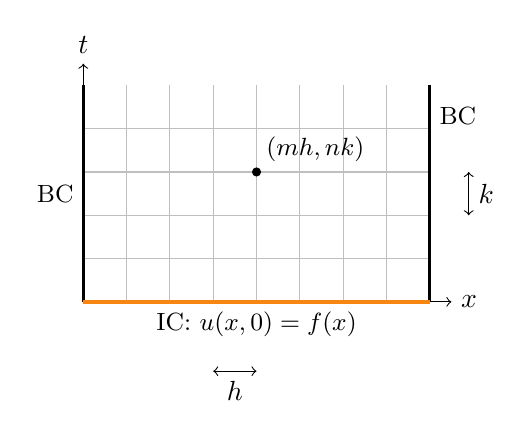
\begin{tikzpicture}[scale=0.55]
\draw[->] (0,0)--(8.5,0) node[right]{\(x\)};
\draw[->] (0,0)--(0,5.5) node[above]{\(t\)};
\foreach \x in {1,...,7} \draw[gray!50] (\x,0)--(\x,5);
\foreach \y in {1,...,4} \draw[gray!50] (0,\y)--(8,\y);
\draw[very thick] (0,0)--(0,5); \draw[very thick] (8,0)--(8,5);
\draw[very thick,BurntOrange] (0,0)--(8,0);
\node[below] at (4,0) {\small IC: \(u(x,0)=f(x)\)};
\node[left] at (0,2.5) {\small BC};
\node[right] at (8,4.3) {\small BC};
\draw[<->] (3,-1.6)--(4,-1.6) node[midway,below]{\(h\)};
\draw[<->] (8.9,2)--(8.9,3) node[midway,right]{\(k\)};
\fill (4,3) circle (3pt) node[above right]{\small\((mh,nk)\)};
\end{tikzpicture}
\end{center}

\subsection{Difference operators}

\begin{definition}[Shift, central difference and derivative operators]
\[
\begin{gathered}
  E f(x)=f(x+h),
  \\
  \delta f(x)=f\bigl(x+\tfrac h2\bigr)-f\bigl(x-\tfrac h2\bigr),
  \\
  Df(x)=f'(x).
\end{gathered}
\]
So \(\delta=E^{1/2}-E^{-1/2}\), and in particular
\[
\begin{gathered}
  \delta^2U_m=U_{m+1}-2U_m+U_{m-1},
  \\
  \delta^4U_m=U_{m+2}-4U_{m+1}+6U_m-4U_{m-1}+U_{m-2}.
\end{gathered}
\]
\end{definition}

\begin{keybox}
\begin{proposition}\label{prop:sinh}
\[
\begin{gathered}
  E=e^{hD},
  \\
  D=\frac2h\sinh^{-1}\frac\delta2,
  \\
  D^2=\frac1{h^2}\Bigl[\delta^2-\frac1{12}\delta^4+\frac1{90}\delta^6
      -\cdots\Bigr].
\end{gathered}
\]
\end{proposition}
\end{keybox}

\begin{proof}\leavevmode
\step{Step 1: \(E=e^{hD}\)}
By Taylor's theorem,
\[
  Ef(x)=f(x+h)
  =\sum_{j\ge0}\frac{h^j}{j!}f^{(j)}(x)
  =\sum_{j\ge0}\frac{(hD)^j}{j!}f(x)
  =e^{hD}f(x).
\]

\step{Step 2: \(\delta\) in terms of \(D\)}

\[
  \delta=E^{1/2}-E^{-1/2}=e^{hD/2}-e^{-hD/2}=2\sinh\frac{hD}{2}
  \quad\Longrightarrow\quad
  D=\frac2h\sinh^{-1}\frac\delta2 .
\]

\step{Step 3: expand}
Using
\[
  \sinh^{-1}z=z-\frac12\frac{z^3}{3}+\frac{1\cdot3}{2\cdot4}\frac{z^5}{5}-\cdots
\]
with \(z=\delta/2\),
\[
  D=\frac1h\Bigl(\delta-\frac{1^2}{2^2\,3!}\delta^3
     +\frac{1^2\,3^2}{2^4\,5!}\delta^5-\cdots\Bigr)
   =\frac1h\Bigl(\delta-\frac{\delta^3}{24}+\frac{3\delta^5}{640}-\cdots\Bigr).
\]

\step{Step 4: square}

\[
  D^2=\frac1{h^2}\Bigl(\delta^2-\frac2{24}\delta^4
      +\Bigl(\frac1{576}+\frac{6}{640}\Bigr)\delta^6-\cdots\Bigr)
     =\frac1{h^2}\Bigl[\delta^2-\frac1{12}\delta^4+\frac1{90}\delta^6
      -\cdots\Bigr].
\]
Keeping only the first term gives the familiar approximation
\(D^2\approx \delta^2/h^2\).
\end{proof}

\begin{remark}
\leavevmode
\begin{itemize}
  \item The series in Step 3 can be written in two ways:
    \[
      \sinh^{-1}z
      =z-\frac12\frac{z^3}{3}+\frac{1\cdot3}{2\cdot4}\frac{z^5}{5}-\cdots
      =z-\frac{1^2}{3!}z^3+\frac{1^2\,3^2}{5!}z^5-\cdots;
    \]
    the coefficients are equal (\(\frac16\) and \(\frac3{40}\)).
  \item In logarithmic form,
    \(\sinh^{-1}z=\ln\bigl(z+\sqrt{z^2+1}\bigr)\).  With \(z=\delta/2\),
    \(\frac\delta2+\sqrt{1+\frac{\delta^2}4}=E^{1/2}\), so
    \(D=\frac2h\ln E^{1/2}=\frac1h\ln E\), which is Step 1 again.  The
    \(\sinh^{-1}\) form is used because it gives a series in powers of
    the \emph{central} difference \(\delta\).
  \item This is the operator (symbolic) method of the calculus of
    finite differences.  The dropped \(-\frac1{12}\delta^4\) term is
    the source of the \(kh^2\) part of the truncation errors below,
    and the same expansion gives Numerov's method:
    \(\delta^2\approx h^2D^2\bigl(1+\frac1{12}\delta^2\bigr)\).
\end{itemize}
\end{remark}

\subsection{Two-level schemes: the key idea}

\begin{definition}[Two-level scheme]
A difference scheme that involves only two adjacent time levels,
\(t_n\) and \(t_{n+1}\), is a \emph{two-level scheme}.  Such schemes
come from the Taylor expansion in \(t\).
\end{definition}

If \(L\) does not depend on \(t\), then \(u_t=Lu\) implies
\(\partial_t^ju=L^ju\).  By Taylor's theorem in \(t\),
\[
  u(x,t+k)
  =\Bigl(1+k\pd{}{t}+\frac{k^2}{2}\pdd{}{t}+\cdots\Bigr)u(x,t)
  =\exp\Bigl(k\pd{}{t}\Bigr)u
  =\exp(kL)\,u,
\]
that is,
\begin{equation}\label{eq:expkl}
  \boxed{u_m^{n+1}=\exp(kL)\,u_m^n}.
\end{equation}
This is \emph{exact}.  Every scheme below comes from
\begin{enumerate}[label=(\alph*)]
  \item writing \(L\) in terms of \(D\),
  \item replacing \(D\) by its series in \(\delta\), and
  \item truncating the expansion.
\end{enumerate}

\subsection{Explicit schemes}

\begin{definition}[Explicit scheme]
An explicit formula involves only \emph{one} grid point at the advanced
time level \(t_{n+1}\).  Each \(U_m^{n+1}\) is computed directly from
known values.
\end{definition}

\subsubsection*{Constant coefficients: \(u_t=u_{xx}\) (\(L=D^2\))}

\begin{proposition}[Explicit schemes]\label{prop:explicit}
For \(u_t=u_{xx}\),
\begin{equation}\label{eq:expseries}
  u_m^{n+1}=\Bigl[1+r\delta^2+\tfrac12r\bigl(r-\tfrac16\bigr)\delta^4
  +\tfrac16r\bigl(r^2-\tfrac12r+\tfrac1{15}\bigr)\delta^6+\cdots\Bigr]u_m^n .
\end{equation}
Keeping only \(\delta^2\) gives the classical explicit scheme
\begin{equation}\label{eq:explicit}
  \boxed{U_m^{n+1}=(1-2r)\,U_m^n+r\,\bigl(U_{m+1}^n+U_{m-1}^n\bigr)},
\end{equation}
and keeping \(\delta^2\) and \(\delta^4\) gives the five-point explicit
scheme
\[
  U_m^{n+1}
  =\tfrac12\bigl(2-5r+6r^2\bigr)U_m^n
   +\tfrac23r(2-3r)\bigl(U_{m+1}^n+U_{m-1}^n\bigr)
   -\tfrac1{12}r(1-6r)\bigl(U_{m+2}^n+U_{m-2}^n\bigr).
\]
\end{proposition}

\begin{proof}
From \eqref{eq:expkl} and Proposition~\ref{prop:sinh}, using
\(k/h^2=r\),
\[
  u_m^{n+1}=\exp(kD^2)u_m^n
  =\exp\Bigl[r\Bigl(\delta^2-\tfrac1{12}\delta^4+\tfrac1{90}\delta^6
   -\cdots\Bigr)\Bigr]u_m^n.
\]
Expand \(e^X=1+X+\frac{X^2}{2}+\frac{X^3}{6}+\cdots\) and collect
powers of \(\delta\):
\begin{align*}
  \delta^2&:\ r,\\
  \delta^4&:\ -\tfrac{r}{12}+\tfrac{r^2}{2}=\tfrac12r\bigl(r-\tfrac16\bigr),\\
  \delta^6&:\ \tfrac{r}{90}-\tfrac{r^2}{12}+\tfrac{r^3}{6}
    =\tfrac16r\bigl(r^2-\tfrac12r+\tfrac1{15}\bigr).
\end{align*}
This is \eqref{eq:expseries}.

\step{(a) Keep only \(\delta^2\)}

\[
  U_m^{n+1}=(1+r\delta^2)U_m^n
  =U_m^n+r\bigl(U_{m+1}^n-2U_m^n+U_{m-1}^n\bigr),
\]
which is \eqref{eq:explicit}.

\step{(b) Keep \(\delta^2\) and \(\delta^4\)}
Write
\(c=\frac12r(r-\frac16)\), expand \(\delta^4U_m\) and collect terms:
\begin{align*}
  U_m:&\quad 1-2r+6c=\tfrac12\bigl(2-5r+6r^2\bigr),\\
  U_{m\pm1}:&\quad r-4c=\tfrac23r(2-3r),\\
  U_{m\pm2}:&\quad c=-\tfrac1{12}r(1-6r).
\end{align*}
Check: the coefficients add to \(1\), as they must, since a constant is
an exact solution.
\end{proof}

\subsubsection*{Variable coefficient: \(u_t=a(x)\,u_{xx}\) (\(L=aD^2\))}

Here
\[
\begin{gathered}
  u_m^{n+1}=\Bigl[1+k\,aD^2+\tfrac12k^2\,aD^2(aD^2)+\cdots\Bigr]u_m^n,
  \\
  aD^2(aD^2)=a\bigl(a''D^2+2a'D^3+aD^4\bigr),
\end{gathered}
\]
where \('\) means \(d/dx\).  The second identity is the product rule
applied twice: \(D^2(a\,D^2u)=a''D^2u+2a'D^3u+aD^4u\).  Keeping the
\(O(k)\) term and replacing \(D^2\approx\delta^2/h^2\),
\[
  U_m^{n+1}=(1+r\,a\,\delta^2)U_m^n
  =\boxed{(1-2ra)U_m^n+ra\bigl(U_{m+1}^n+U_{m-1}^n\bigr)},
  \qquad a=a(mh).
\]

\subsubsection*{Self-adjoint form: \(u_t=\partial_x\bigl(a(x)\,u_x\bigr)\)}

Expanding, \(u_t=a'u_x+a\,u_{xx}\), so \(L=a'D+aD^2\) and
\[
  u_m^{n+1}=\exp\bigl(k(a'D+aD^2)\bigr)u_m^n
  =\bigl[1+k(a'D+aD^2)+\cdots\bigr]u_m^n.
\]
Neglect terms of order \(k^2\) and above, and replace (central
differences)
\[
\begin{gathered}
  D^2U_m\approx\frac1{h^2}\delta^2U_m,
  \\
  DU_m\approx\frac1{2h}\bigl(U_{m+1}-U_{m-1}\bigr).
\end{gathered}
\]
Then
\[
  U_m^{n+1}=U_m^n+k\Bigl[\frac{a'}{2h}\bigl(U_{m+1}^n-U_{m-1}^n\bigr)
  +\frac{a}{h^2}\bigl(U_{m+1}^n-2U_m^n+U_{m-1}^n\bigr)\Bigr],
\]
so
\[
  \boxed{U_m^{n+1}=(1-2ra)U_m^n+r\bigl(a+\tfrac12ha'\bigr)U_{m+1}^n
  +r\bigl(a-\tfrac12ha'\bigr)U_{m-1}^n},
\]
with \(a\) and \(a'\) evaluated at \(x=mh\).

\begin{exercise}
Repeat this derivation for \(u_t=\partial_x\bigl(a(x,t)\,u_x\bigr)\).
\end{exercise}

\subsection{Implicit schemes: Crank--Nicolson}

\begin{definition}[Implicit scheme]
An implicit formula involves \emph{more than one} grid point at the
advanced time level.  A linear system (here tridiagonal) must be
solved at each step.
\end{definition}

\begin{proposition}[Crank--Nicolson scheme]\label{prop:cn}
For \(u_t=u_{xx}\), the Crank--Nicolson scheme is
\begin{equation}\label{eq:cn}
  \boxed{\bigl(1-\tfrac12r\delta^2\bigr)U_m^{n+1}
  =\bigl(1+\tfrac12r\delta^2\bigr)U_m^n},
\end{equation}
that is,
\begin{equation}\label{eq:cn2}
  (1+r)U_m^{n+1}-\tfrac12r\bigl(U_{m+1}^{n+1}+U_{m-1}^{n+1}\bigr)
  =(1-r)U_m^n+\tfrac12r\bigl(U_{m+1}^n+U_{m-1}^n\bigr).
\end{equation}
Its principal error term is \(O(k^3+kh^2)\).
\end{proposition}

\begin{proof}
Split \eqref{eq:expkl} symmetrically about \(t_{n+1/2}\):
\[
  u_m^{n+1}=\exp(kL)u_m^n
  \iff
  \exp\bigl(-\tfrac12kL\bigr)u_m^{n+1}=\exp\bigl(\tfrac12kL\bigr)u_m^n.
\]
For \(u_t=u_{xx}\) (\(L=D^2\)),
\[
  \exp\bigl(-\tfrac12kD^2\bigr)u_m^{n+1}=\exp\bigl(\tfrac12kD^2\bigr)u_m^n.
\]
Put \(D^2\approx\delta^2/h^2\) and keep the first two terms of each
exponential; this gives \eqref{eq:cn}.  Written out,
\[
  U_m^{n+1}-\tfrac12r\bigl(U_{m+1}^{n+1}-2U_m^{n+1}+U_{m-1}^{n+1}\bigr)
  =U_m^n+\tfrac12r\bigl(U_{m+1}^n-2U_m^n+U_{m-1}^n\bigr),
\]
which rearranges to \eqref{eq:cn2}.

Because the splitting is symmetric about \(t_{n+1/2}\), the \(k^2\)
terms cancel, leaving \(O(k^3)\).  The \(kh^2\) term comes from
dropping \(-\frac1{12}\delta^4\) in \(D^2\).
\end{proof}

\begin{center}
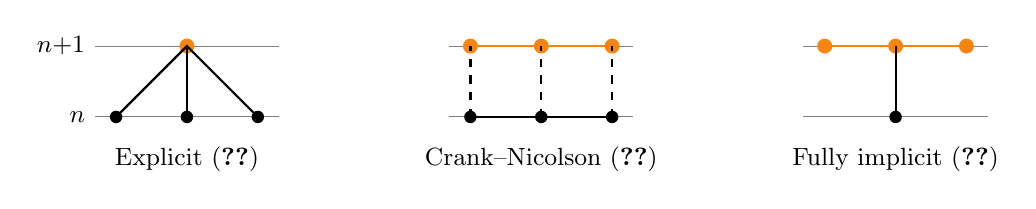
\begin{tikzpicture}[scale=0.9,every node/.style={font=\small}]
\begin{scope}
\draw[gray] (-1.3,0)--(1.3,0); \draw[gray] (-1.3,1)--(1.3,1);
\foreach \x in {-1,0,1} \fill (\x,0) circle (2.5pt);
\fill[BurntOrange] (0,1) circle (3pt);
\draw[thick] (-1,0)--(0,1)--(1,0); \draw[thick] (0,0)--(0,1);
\node at (0,-0.6) {Explicit \eqref{eq:explicit}};
\node[left] at (-1.3,0){\(n\)}; \node[left] at (-1.3,1){\(n{+}1\)};
\end{scope}
\begin{scope}[xshift=5cm]
\draw[gray] (-1.3,0)--(1.3,0); \draw[gray] (-1.3,1)--(1.3,1);
\foreach \x in {-1,0,1} {\fill (\x,0) circle (2.5pt); \fill[BurntOrange] (\x,1) circle (3pt);}
\draw[thick] (-1,0)--(1,0); \draw[thick,BurntOrange] (-1,1)--(1,1);
\foreach \x in {-1,0,1} \draw[thick,dashed] (\x,0)--(\x,1);
\node at (0,-0.6) {Crank--Nicolson \eqref{eq:cn2}};
\end{scope}
\begin{scope}[xshift=10cm]
\draw[gray] (-1.3,0)--(1.3,0); \draw[gray] (-1.3,1)--(1.3,1);
\fill (0,0) circle (2.5pt);
\foreach \x in {-1,0,1} \fill[BurntOrange] (\x,1) circle (3pt);
\draw[thick,BurntOrange] (-1,1)--(1,1); \draw[thick] (0,0)--(0,1);
\node at (0,-0.6) {Fully implicit \eqref{eq:impl}};
\end{scope}
\end{tikzpicture}

\small Computational stencils.  Orange points are unknowns at the new
time level.
\end{center}

\subsection{Local truncation error and consistency}

\begin{definition}[Local truncation error]
The local truncation error (LTE) \(T_m^n\) is what remains when the
\emph{exact} solution \(u\) of the PDE is substituted into the
difference scheme.
\end{definition}

\begin{proposition}[LTE of the explicit scheme]\label{prop:lte}
For the explicit scheme \eqref{eq:explicit},
\[
  T_m^n
  =\tfrac12k^2\Bigl(\pdd ut-\frac1{6r}\frac{\partial^4u}{\partial x^4}\Bigr)_m^n
   +\cdots
  =O(k^2+kh^2).
\]
\end{proposition}

\begin{proof}
By definition,
\[
  T_m^n=u_m^{n+1}-(1-2r)u_m^n-r\bigl(u_{m+1}^n+u_{m-1}^n\bigr).
\]
Taylor-expand about \((mh,nk)\), with all derivatives evaluated there:
\begin{align*}
  u_m^{n+1}&=u+k\,u_t+\tfrac12k^2u_{tt}+\tfrac16k^3u_{ttt}+\cdots,\\
  u_{m\pm1}^n&=u\pm h\,u_x+\tfrac12h^2u_{xx}\pm\tfrac16h^3u_{xxx}
    +\tfrac1{24}h^4u_{xxxx}\pm\cdots.
\end{align*}
Adding the two space expansions, the odd terms cancel:
\[
  u_{m+1}^n+u_{m-1}^n=2u+h^2u_{xx}+\tfrac1{12}h^4u_{xxxx}+\cdots.
\]
Multiply by \(r\) and use \(rh^2=k\):
\[
  r\bigl(u_{m+1}^n+u_{m-1}^n\bigr)
  =2ru+k\,u_{xx}+\tfrac{1}{12}kh^2u_{xxxx}+\cdots.
\]
Substituting, the \(u\) terms cancel since \(1-(1-2r)-2r=0\), and
\[
  T_m^n=k\bigl(u_t-u_{xx}\bigr)+\tfrac12k^2u_{tt}
        -\tfrac1{12}kh^2u_{xxxx}+\cdots.
\]
Since \(u_t=u_{xx}\) and \(kh^2=k^2/r\), the result follows.
\end{proof}

The quantity
\(\frac12k^2\bigl(u_{tt}-\frac1{6r}u_{xxxx}\bigr)\) is the
\emph{principal part} of the LTE.  Because \(u_{tt}=u_{xxxx}\) for the
heat equation, choosing \(r=\frac16\) makes it vanish, giving a
higher-order scheme.  This agrees with \eqref{eq:expseries}: the
\(\delta^4\) coefficient \(\frac12r(r-\frac16)\) is zero when
\(r=\frac16\).

\begin{definition}[Consistency]
A finite difference scheme is \emph{consistent} with the PDE if
\[
  \frac{T_m^n}{k}\to0\quad\text{as }h,k\to0.
\]
\end{definition}

For the explicit scheme, \(T/k=O(k+h^2)\to0\), so it is consistent.

\step{The error equation}
Let \(z_m^n=u_m^n-U_m^n\).  The exact
solution satisfies
\[
  u_m^{n+1}=(1-2r)u_m^n+r(u_{m+1}^n+u_{m-1}^n)+T_m^n,
\]
while \(U\) satisfies the same equation with \(T=0\).  Subtracting,
\begin{equation}\label{eq:erreq}
  z_m^{n+1}=(1-2r)z_m^n+r\bigl(z_{m+1}^n+z_{m-1}^n\bigr)+T_m^n,
  \qquad T_m^n=O(k^2+kh^2).
\end{equation}

\section{Convergence}

\begin{definition}[Convergence]
Let \(\pd ut=L(x,t,D,D^2)u\).  The problem of convergence of a finite
difference scheme is to find conditions under which
\[
  u(X,T)-U(X,T)\to0,\qquad X=mh,\ T=nk,
\]
at a \emph{fixed} point \((X,T)\), uniformly, as the mesh is refined so
that \(h,k\to0\) and \(m,n\to\infty\) with \(X=mh\) and \(T=nk\) fixed.
The point \((X,T)\) may be anywhere in the region \(R\) under
consideration.
\end{definition}

\begin{keybox}
\begin{theorem}\label{thm:conv-explicit}
For \(u_t=u_{xx}\) on \(0\le x\le1\) with Dirichlet boundary
conditions, the explicit scheme \eqref{eq:explicit} is convergent
whenever \(0<r\le\frac12\).  More precisely,
\[
  \max_m|u_m^n-U_m^n|\le T\,A\,(k+h^2),\qquad T=nk,
\]
where \(A\) depends only on bounds for \(u_{tt}\) and \(u_{xxxx}\).
\end{theorem}
\end{keybox}

\begin{proof}
The error \(z_m^n=u_m^n-U_m^n\) satisfies \eqref{eq:erreq}, with
\(z_0^n=z_N^n=0\) because of the Dirichlet conditions.

\step{Step 1: bound the LTE}
Taylor's theorem with remainder gives
\[
  T_m^n=\tfrac12k^2\,u_{tt}(mh,\,nk+\theta_1k)
        -\tfrac1{12}kh^2\,u_{xxxx}(mh+\theta_2h,\,nk),
  \qquad |\theta_i|<1.
\]
If \(|u_{tt}|\le M_{tt}\) and \(|u_{xxxx}|\le M_{xxxx}\) in \(R\), then
\[
  |T_m^n|\le A\,(k^2+kh^2),
  \qquad A=\max\bigl(\tfrac12M_{tt},\tfrac1{12}M_{xxxx}\bigr).
\]

\step{Step 2: use \(r\le\frac12\)}
If \(0<r\le\frac12\), all
coefficients \(1-2r,\ r,\ r\) on the right of \eqref{eq:erreq} are
\emph{non-negative}, so
\[
  |z_m^{n+1}|\le(1-2r)|z_m^n|+r|z_{m+1}^n|+r|z_{m-1}^n|+A(k^2+kh^2).
\]
Let \(Z^{(n)}=\max_{0\le m\le N}|z_m^n|\), the maximum error on time
level \(n\).  Each \(|z_j^n|\le Z^{(n)}\), and the coefficients sum to
\((1-2r)+r+r=1\), so
\[
  |z_m^{n+1}|\le Z^{(n)}+A(k^2+kh^2)\quad\text{for every }m,
\]
hence
\[
  Z^{(n+1)}\le Z^{(n)}+A(k^2+kh^2).
\]

\step{Step 3: iterate}

\begin{align*}
  Z^{(n)}&\le Z^{(n-1)}+A(k^2+kh^2)\le Z^{(n-2)}+2A(k^2+kh^2)\le\cdots\\
  &\le Z^{(0)}+nA(k^2+kh^2)=Z^{(0)}+nk\,A\,(k+h^2).
\end{align*}

\step{Step 4: conclude}
The PDE and the difference equation use the
same initial data, so \(Z^{(0)}=0\).  With \(nk=T\),
\[
  Z^{(n)}\le T\,A\,(k+h^2)\longrightarrow0
  \qquad\text{as }h,k\to0,\ \text{for fixed }X,T. \qedhere
\]
\end{proof}

\begin{remark}[Why the proof needs \(r\le\frac12\)]
If \(r>\frac12\), then \(1-2r<0\) and the triangle-inequality step no
longer closes the bound, because the absolute values of the
coefficients add to \(|1-2r|+2r=4r-1>1\).  This is not just a gap in
the proof: the stability analysis below shows that the scheme really
does blow up for \(r>\frac12\).
\end{remark}

\section{Stability}

\begin{keybox}
\begin{theorem}[Lax equivalence theorem]\label{thm:lax}
Given a properly posed linear initial value problem and a finite
difference approximation to it that satisfies the consistency
condition, stability is the necessary and sufficient condition for
convergence:
\[
  \text{consistency}+\text{stability}\iff\text{convergence}.
\]
\end{theorem}
\end{keybox}

So in practice we check consistency (from the LTE) and stability.  This
is often much easier than proving convergence directly, as in
Theorem~\ref{thm:conv-explicit}.

\begin{definition}[Stability]
The problem of stability of a finite difference method is to find
conditions under which the difference
\[
  z_m^n=U_m^n-\widetilde U_m^n
\]
between the theoretical solution \(U\) and the numerical solution
\(\widetilde U\) of the \emph{difference} equation (for example,
\(\widetilde U\) carries round-off errors) stays bounded as
\(n\to\infty\).  For the Lax equivalence theorem the bound must hold
uniformly as the mesh is refined (\(h,k\to0\), \(nk\le T\)); this is made
precise by the Lax--Richtmyer definition in the matrix method below.
\end{definition}

Methods for analysing stability: (1) the von Neumann (Fourier) method,
(2) the matrix method, (3) the energy method.

\subsection{The von Neumann (Fourier) method}

\step{Idea}
For a linear scheme with constant coefficients, the
error \(z\) satisfies the \emph{same} difference equation as \(U\).
Expand the initial error on the grid in a finite Fourier series
(harmonic decomposition):
\[
  z_m^0=\sum_jA_j\,e^{i\beta_jmh}.
\]
By linearity each harmonic evolves on its own, so it is enough to
follow one term.  Look for a solution of the form
\[
  z_m^n=e^{\alpha nk}\,e^{i\beta mh}=\xi^n\,e^{i\beta mh},
  \qquad \xi=e^{\alpha k}.
\]
At \(t=0\) this is just \(e^{i\beta x}\); after \(n\) steps it has been
multiplied by \(\xi^n=(e^{\alpha k})^n\).

\begin{definition}[Amplification factor]
\(\xi=e^{\alpha k}\) is the \emph{growth} (or \emph{amplification})
factor.  The von Neumann condition for stability is
\[
  |\xi|\le1\quad\text{for all }\beta,
  \qquad\text{i.e. } |e^{\alpha k}|\le1.
\]
\end{definition}

\begin{keybox}
\begin{theorem}[Explicit scheme]\label{thm:vn1}
The amplification factor of the explicit scheme \eqref{eq:explicit} is
\[
  \xi=1-4r\sin^2\frac{\beta h}2,
\]
and the scheme is stable if and only if \(0<r\le\frac12\)
(conditionally stable).
\end{theorem}
\end{keybox}

\begin{proof}
The perturbed solution \(\widetilde U\) satisfies the same scheme, so
the error satisfies
\[
  z_m^{n+1}=(1-2r)z_m^n+r\bigl(z_{m+1}^n+z_{m-1}^n\bigr).
\]
Substitute \(z_m^n=e^{\alpha nk}e^{i\beta mh}\):
\[
  e^{\alpha(n+1)k}e^{i\beta mh}
  =(1-2r)e^{\alpha nk}e^{i\beta mh}
   +r\,e^{\alpha nk}\bigl(e^{i\beta(m+1)h}+e^{i\beta(m-1)h}\bigr).
\]
Dividing by \(e^{\alpha nk}e^{i\beta mh}\),
\[
  \xi=e^{\alpha k}
  =(1-2r)+r\bigl(e^{i\beta h}+e^{-i\beta h}\bigr)
  =(1-2r)+2r\cos\beta h.
\]
Using \(\cos\beta h=1-2\sin^2\frac{\beta h}{2}\),
\[
  \boxed{\xi=1-4r\sin^2\frac{\beta h}2}.
\]
For stability we need \(|\xi|\le1\), i.e.
\[
  -1\le1-4r\sin^2\frac{\beta h}2\le1.
\]
The right-hand inequality holds trivially for \(r>0\).  The left-hand
one gives
\[
  4r\sin^2\frac{\beta h}2\le2
  \iff
  r\le\frac1{2\sin^2(\beta h/2)}\quad\text{for all }\beta.
\]
The worst case is \(\sin^2=1\), so
\[
  \boxed{0<r\le\tfrac12}. \qedhere
\]
\end{proof}

\begin{keybox}
\begin{theorem}[Fully implicit scheme]\label{thm:vn2}
The fully implicit scheme
\begin{equation}\label{eq:impl}
  \frac{U_m^{n+1}-U_m^n}{k}
  =\frac{U_{m+1}^{n+1}-2U_m^{n+1}+U_{m-1}^{n+1}}{h^2}
  \iff
  -rU_{m-1}^{n+1}+(1+2r)U_m^{n+1}-rU_{m+1}^{n+1}=U_m^n
\end{equation}
has amplification factor
\[
  \xi=\frac{1}{1+4r\sin^2(\beta h/2)},
\]
and is unconditionally stable.
\end{theorem}
\end{keybox}

\begin{proof}
Substitute \(z_m^n=\xi^ne^{i\beta mh}\) into \eqref{eq:impl} and divide
by \(\xi^ne^{i\beta mh}\):
\[
  \xi\bigl[(1+2r)-2r\cos\beta h\bigr]=1
  \quad\Longrightarrow\quad
  \xi\Bigl[1+4r\sin^2\frac{\beta h}2\Bigr]=1
  \quad\Longrightarrow\quad
  \boxed{\xi=\frac{1}{1+4r\sin^2(\beta h/2)}}.
\]
Then \(0<\xi\le1\) for every \(r>0\) and every \(\beta\), so the scheme
is unconditionally stable.
\end{proof}

\begin{remark}[Crank--Nicolson by von Neumann]
Substituting into \eqref{eq:cn2} gives
\[
  \xi=\frac{1-2r\sin^2(\beta h/2)}{1+2r\sin^2(\beta h/2)},
\]
so \(|\xi|\le1\) for all \(r>0\), and Crank--Nicolson is
unconditionally stable.  The matrix method below gives the same
result.
\end{remark}

\subsection{The matrix method}

Here we work on \([0\le x\le1]\times[0\le t\le T]\) with constant
coefficients.  The grid is \(x_i=ih\) for \(i=0,\dots,N\), with
\(Nh=1\), and \(t_j=jk\).  Here \(h\) and \(k\) are related, for example
\(k=rh^2\) with \(r>0\) fixed, so \(k\to0\) as \(h\to0\).

Assume the two-level scheme relating the mesh values on time levels
\(j+1\) and \(j\) is
\[
  b_{i-1}U_{i-1}^{j+1}+b_iU_i^{j+1}+b_{i+1}U_{i+1}^{j+1}
  =c_{i-1}U_{i-1}^j+c_iU_i^j+c_{i+1}U_{i+1}^j,
\]
with constant coefficients.  If the boundary values at \(i=0\) and
\(i=N\) are known for \(j>0\), the \(N-1\) equations for
\(i=1,\dots,N-1\) form the matrix system
\[
  B\,\mathbf U_{j+1}=C\,\mathbf U_j+\mathbf d_j,
  \qquad \mathbf U_j=\bigl(U_1^j,\dots,U_{N-1}^j\bigr)^T.
\]
Here \(B\) and \(C\) are tridiagonal, and \(\mathbf d_j\) holds the
known boundary values: its first entry is \(c_0U_0^j-b_0U_0^{j+1}\), its
last entry is \(c_NU_N^j-b_NU_N^{j+1}\), and all other entries are zero.
Hence
\[
  \mathbf U_{j+1}=B^{-1}C\,\mathbf U_j+B^{-1}\mathbf d_j
  =A\,\mathbf U_j+\mathbf f_j,
  \qquad A=B^{-1}C,\quad \mathbf f_j=B^{-1}\mathbf d_j.
\]

\begin{definition}[Lax--Richtmyer stability]
The scheme is \emph{stable} if there is a positive number \(M\),
independent of \(j\), \(h\) and \(k\), such that
\[
  \|A^j\|\le M,\qquad j=1,\dots,J\ \ (jk\le T).
\]
\end{definition}

\begin{keybox}
\begin{theorem}[Matrix method]\label{thm:matrix}
\leavevmode
\begin{enumerate}[label=(\alph*)]
  \item A perturbation \(\mathbf e_0\) of the initial values propagates
    as \(\mathbf e_j=A^j\mathbf e_0\), so
    \(\|\mathbf e_j\|\le\|A^j\|\,\|\mathbf e_0\|\).
  \item If \(\|A\|\le1\), the scheme is Lax--Richtmyer stable (with
    \(M=1\)).
  \item If \(A\) is real and symmetric, then \(\|A^j\|_2=\rho(A)^j\), so
    \(\rho(A)\le1\) gives stability (with \(M=1\)), while the powers
    grow without bound if \(\rho(A)\) exceeds \(1\) by a fixed amount.
\end{enumerate}
\end{theorem}
\end{keybox}

\begin{proof}\leavevmode
\step{Step 1: solve the recursion}
Applying
\(\mathbf U_{j}=A\mathbf U_{j-1}+\mathbf f_{j-1}\) repeatedly,
\begin{align}
  \mathbf U_j
  &=A\mathbf U_{j-1}+\mathbf f_{j-1}
   =A\bigl(A\mathbf U_{j-2}+\mathbf f_{j-2}\bigr)+\mathbf f_{j-1}
   =A^2\mathbf U_{j-2}+A\mathbf f_{j-2}+\mathbf f_{j-1}
   =\cdots\notag\\
  &=A^j\mathbf U_0+A^{j-1}\mathbf f_0+A^{j-2}\mathbf f_1+\cdots
    +\mathbf f_{j-1}. \label{eq:mat1}
\end{align}
Here \(\mathbf U_0\) is the vector of initial values, and
\(\mathbf f_0,\dots,\mathbf f_{j-1}\) come from the known boundary
values.

\step{Step 2: perturb the initial data}
Replace \(\mathbf U_0\) by
\(\mathbf U_0^*\), for example because of rounding.  The solution at
time row \(j\) becomes
\begin{equation}\label{eq:mat2}
  \mathbf U_j^*=A^j\mathbf U_0^*+A^{j-1}\mathbf f_0+\cdots
                +\mathbf f_{j-1}.
\end{equation}
Define the error vector \(\mathbf e_j=\mathbf U_j^*-\mathbf U_j\).
Subtracting \eqref{eq:mat1} from \eqref{eq:mat2}, the \(\mathbf f\)
terms cancel:
\[
  \boxed{\mathbf e_j=A^j\bigl(\mathbf U_0^*-\mathbf U_0\bigr)
         =A^j\mathbf e_0},
  \qquad\text{equivalently }\ \mathbf e_j=A\mathbf e_{j-1}.
\]
So a perturbation \(\mathbf e_0\) of the initial values is propagated
by powers of \(A\).

\step{Step 3: take norms}
For a compatible matrix and vector norm,
\(\|\mathbf e_j\|\le\|A^j\|\,\|\mathbf e_0\|\).  Under Lax--Richtmyer
stability, \(\|\mathbf e_j\|\le M\|\mathbf e_0\|\): the amplification
of any initial perturbation, and so of any initial rounding error, is
limited.  This proves (a).

\step{Step 4: a sufficient condition}
By submultiplicativity,
\[
  \|A^j\|=\|A\,A^{j-1}\|\le\|A\|\,\|A^{j-1}\|\le\cdots\le\|A\|^j.
\]
So
\[
  \boxed{\|A\|\le1}\ \Longrightarrow\ \|A^j\|\le1,
\]
which is Lax--Richtmyer stability with \(M=1\).  This proves (b).  The
condition \(\|A\|\le1\) is the natural requirement when the solution of
the PDE does not increase as \(t\) increases: it is necessary and
sufficient for the strong bound \(\|A^j\|\le1\) for all \(j\) (take
\(j=1\)).  It is \emph{not} necessary for Lax--Richtmyer stability with
some larger \(M\); see the example below.

\step{Step 5: the spectral radius}
Let \(\rho(A)=\max_i|\lambda_i|\).
Since \(\rho(A)\le\|A\|\) for every norm, \(\|A\|\le1\) implies
\(\rho(A)\le1\).  The converse is \emph{false} in general:
\(\rho(A)\le1\) does not imply \(\|A\|\le1\).  If, however, \(A\) is
real and symmetric, the spectral norm satisfies
\[
  \|A\|_2=\sqrt{\rho(A^TA)}=\sqrt{\rho(A^2)}=\sqrt{\rho(A)^2}=\rho(A).
\]
Hence \(\|A^j\|_2=\rho(A)^j\), so for symmetric \(A\) the condition
\(\rho(A)\le1\) gives stability with \(M=1\), and it is the condition
used in practice.  (Strictly, over a finite time \(jk\le T\) a bound
\(\rho(A)\le1+O(k)\) would also keep \(\|A^j\|\) bounded, by
\(e^{O(T)}\).)  This proves (c).
\end{proof}

\begin{example}[\(\rho(A)<1\) but \(\|A\|>1\)]
Let
\[
  A=\begin{pmatrix}-0.8&0\\0.4&0.7\end{pmatrix}.
\]
Its eigenvalues are \(\lambda_1=-0.8\) and \(\lambda_2=0.7\), so
\(\rho(A)=0.8\).  But \(\|A\|_1=1.2\) (largest column sum) and
\(\|A\|_\infty=1.1\) (largest row sum).  This \(A\) is not symmetric
(not even normal: \(AA^T\ne A^TA\)), so the spectral radius alone does
not control the norm.  Its powers are
still bounded, however: since \(\rho(A)<1\), \(A^j\to0\) (for example
\(\|A^j\|_1\le1.2\) for all \(j\)).  So \(\|A\|\le1\) is sufficient but
not necessary for Lax--Richtmyer stability.
\end{example}

\begin{keybox}
\begin{theorem}[Eigenvalues of a tridiagonal matrix]\label{thm:tridiag}
Let \(A\) be the \(N\times N\) tridiagonal matrix with \(a\) on the
diagonal, \(b\) above it and \(c\) below it, where \(bc\ne0\).  Its
eigenvalues are
\[
  \lambda_s=a+2b\Bigl(\frac cb\Bigr)^{1/2}\cos\frac{s\pi}{N+1},
  \qquad s=1,\dots,N,
\]
with eigenvectors
\[
  \mathbf v_s
  =\Bigl[\Bigl(\tfrac cb\Bigr)^{1/2}\sin\tfrac{s\pi}{N+1},\
         \Bigl(\tfrac cb\Bigr)\sin\tfrac{2s\pi}{N+1},\
         \Bigl(\tfrac cb\Bigr)^{3/2}\sin\tfrac{3s\pi}{N+1},\
         \dots,\
         \Bigl(\tfrac cb\Bigr)^{N/2}\sin\tfrac{Ns\pi}{N+1}\Bigr]^T.
\]
When \(b,c>0\), \(\lambda_s=a+2\sqrt{bc}\,\cos\frac{s\pi}{N+1}\).  For an
\((N-1)\times(N-1)\) matrix, replace \(N+1\) by \(N\) and take
\(s=1,\dots,N-1\).
\end{theorem}
\end{keybox}

The proof is given in Section~\ref{sec:tridiag}.

\begin{keybox}
\begin{theorem}[Matrix stability of the explicit scheme]\label{thm:mexp}
The explicit scheme \eqref{eq:explicit} with Dirichlet boundary
conditions is stable in the matrix sense if and only if
\(0<r\le\frac12\) (for all \(N\)).
\end{theorem}
\end{keybox}

\begin{proof}
For \eqref{eq:explicit} we have \(B=I\) and
\[
  A=C=\begin{pmatrix}1-2r&r&&\\ r&1-2r&r&\\ &\ddots&\ddots&\ddots\\ &&r&1-2r\end{pmatrix}_{(N-1)\times(N-1)}.
\]
By Theorem~\ref{thm:tridiag} with \(a=1-2r\), \(b=c=r\) and size
\(N-1\),
\[
  \lambda_s=(1-2r)+2r\cos\frac{s\pi}N
  =(1-2r)+2r\Bigl(1-2\sin^2\frac{s\pi}{2N}\Bigr)
  =\boxed{1-4r\sin^2\frac{s\pi}{2N}},
  \quad s=1,\dots,N-1.
\]
\(C\) is real and symmetric, so stability holds if and only if
\(\rho(C)\le1\), i.e.
\[
  -1\le1-4r\sin^2\frac{s\pi}{2N}\le1\quad\text{for all }s.
\]
The right-hand inequality holds for all \(r>0\).  The left-hand one
gives
\[
  r\le\frac1{2\sin^2\bigl(s\pi/(2N)\bigr)}.
\]
As \(h\to0\) (\(N\to\infty\)), \(\sin^2\frac{(N-1)\pi}{2N}\to1\), so we
need
\[
  \boxed{0<r\le\tfrac12}.
\]
This is the same as the von Neumann condition.
\end{proof}

\begin{keybox}
\begin{theorem}[Matrix stability of Crank--Nicolson]\label{thm:mcn}
The Crank--Nicolson scheme \eqref{eq:cn2} with Dirichlet boundary
conditions is unconditionally stable, and hence (being consistent)
convergent for every \(r>0\).
\end{theorem}
\end{keybox}

\begin{proof}
Write \eqref{eq:cn2} as \(A\mathbf U^{n+1}=B\mathbf U^n\), so
\(\mathbf U^{n+1}=A^{-1}B\,\mathbf U^n\), with
\[
\begin{gathered}
  A=\mathrm{tridiag}\bigl(-\tfrac r2,\ 1+r,\ -\tfrac r2\bigr),
  \\
  B=\mathrm{tridiag}\bigl(\tfrac r2,\ 1-r,\ \tfrac r2\bigr),
\end{gathered}
\]
both of size \((N-1)\times(N-1)\).  With \(\theta_s=\frac{s\pi}{2N}\),
\(s=1,\dots,N-1\),
\begin{align*}
  \lambda_s(B)&=(1-r)+r\cos\frac{s\pi}N=1-2r\sin^2\theta_s,\\
  \lambda_s(A)&=(1+r)-r\cos\frac{s\pi}N=1+2r\sin^2\theta_s.
\end{align*}

\step{Why we may divide eigenvalues}
Let
\(T_0=\mathrm{tridiag}(1,-2,1)\).  Then
\[
  A=I-\tfrac r2T_0,\qquad B=I+\tfrac r2T_0
\]
are both polynomials in the same symmetric matrix.  So they commute and
share the eigenvectors of \(T_0\).  On a common eigenvector,
\(A^{-1}B\) acts as multiplication by \(\lambda_s(B)/\lambda_s(A)\).
(This is \emph{not} true for general matrices: in general the
eigenvalues of \(A^{-1}B\) are not ratios of eigenvalues.)  Hence
\[
  \boxed{\lambda_s(A^{-1}B)=\frac{1-2r\sin^2\theta_s}{1+2r\sin^2\theta_s}},
  \qquad s=1,\dots,N-1.
\]
Since \(2r\sin^2\theta_s>0\), the numerator has smaller absolute value
than the denominator, so \(|\lambda_s(A^{-1}B)|<1\) for all \(r>0\).
Also, \(A^{-1}B\) is symmetric (a product of commuting symmetric
matrices), so
\[
  \|A^{-1}B\|_2=\rho(A^{-1}B)<1\quad\text{for all } r>0 .
\]
This is unconditional stability.  Since Crank--Nicolson is also
consistent, the Lax equivalence theorem gives convergence for every
\(r>0\).
\end{proof}

\subsection{Eigenvalues and eigenvectors of a tridiagonal
matrix}\label{sec:tridiag}

\begin{proof}[Proof of Theorem~\ref{thm:tridiag}]
Let
\[
  A=\begin{pmatrix}a&b&&\\ c&a&b&\\ &\ddots&\ddots&\ddots\\ &&c&a\end{pmatrix}_{N\times N},
\]
where \(a,b,c\) are real or complex and \(bc\ne0\).

\step{Step 1: a difference equation}
Let \(A\mathbf v=\lambda\mathbf v\)
with \(\mathbf v=(v_1,\dots,v_N)^T\ne0\).  Row by row,
\((A-\lambda I)\mathbf v=0\) reads
\begin{align*}
  (a-\lambda)v_1+bv_2&=0,\\
  cv_{j-1}+(a-\lambda)v_j+bv_{j+1}&=0,\qquad 2\le j\le N-1,\\
  cv_{N-1}+(a-\lambda)v_N&=0.
\end{align*}
Define \(v_0=v_{N+1}=0\).  Then all \(N\) equations combine into one
difference equation with two boundary conditions:
\begin{equation}\label{eq:tri1}
  cv_{j-1}+(a-\lambda)v_j+bv_{j+1}=0,\qquad j=1,\dots,N,
  \qquad v_0=v_{N+1}=0.
\end{equation}

\step{Step 2: general solution}
Try \(v_j=m^j\).  This gives the
auxiliary equation
\begin{equation}\label{eq:tri3}
  bm^2+(a-\lambda)m+c=0.
\end{equation}
With roots \(m_1,m_2\),
\[
  v_j=B\,m_1^j+C\,m_2^j,\qquad B,C\text{ arbitrary constants}.
\]

\step{Step 3: the roots cannot be equal}
If \(m_1=m_2\), then
\(v_j=(B+Cj)m_1^j\).  The condition \(v_0=0\) gives \(B=0\), and
\(v_{N+1}=0\) gives \(C=0\) (note \(m_1\ne0\), because
\(m_1m_2=c/b\ne0\)).  So \(\mathbf v=0\), which is impossible for an
eigenvector.  Hence \(m_1\ne m_2\).

\step{Step 4: apply the boundary conditions}

\[
\begin{gathered}
  v_0=0\ \Rightarrow\ B+C=0\ \Rightarrow\ C=-B,
  \\
  v_{N+1}=0\ \Rightarrow\ Bm_1^{N+1}=-Cm_2^{N+1}=Bm_2^{N+1}.
\end{gathered}
\]
Since \(B\ne0\),
\begin{equation}\label{eq:tri4}
  \Bigl(\frac{m_1}{m_2}\Bigr)^{N+1}=1=e^{2is\pi}
  \quad\Longrightarrow\quad
  \frac{m_1}{m_2}=e^{2is\pi/(N+1)},\qquad s=1,\dots,N.
\end{equation}
(\(s=0\) is excluded because \(m_1\ne m_2\).)  From \eqref{eq:tri3},
the product of the roots is
\begin{equation}\label{eq:tri5}
  m_1m_2=\frac cb.
\end{equation}

\step{Step 5: solve for \(m_1,m_2\)}
Multiplying \eqref{eq:tri4}
and \eqref{eq:tri5} gives \(m_1^2=\frac cb e^{2is\pi/(N+1)}\), so
\[
\begin{gathered}
  m_1=\Bigl(\frac cb\Bigr)^{1/2}e^{is\pi/(N+1)},
  \\
  m_2=\Bigl(\frac cb\Bigr)^{1/2}e^{-is\pi/(N+1)}.
\end{gathered}
\]

\step{Step 6: the eigenvalues}
From \eqref{eq:tri3}, the sum of
the roots is \(m_1+m_2=-\frac{a-\lambda}{b}=\frac{\lambda-a}b\).
Therefore
\[
  \lambda=a+b\Bigl(\frac cb\Bigr)^{1/2}
          \Bigl[e^{is\pi/(N+1)}+e^{-is\pi/(N+1)}\Bigr]
  =a+2b\Bigl(\frac cb\Bigr)^{1/2}\cos\frac{s\pi}{N+1},
  \qquad s=1,\dots,N.
\]

\step{Step 7: the eigenvectors}
With \(C=-B\),
\[
  v_j=B\bigl(m_1^j-m_2^j\bigr)
  =B\Bigl(\frac cb\Bigr)^{j/2}
    \Bigl[e^{ijs\pi/(N+1)}-e^{-ijs\pi/(N+1)}\Bigr]
  =2iB\Bigl(\frac cb\Bigr)^{j/2}\sin\frac{js\pi}{N+1}.
\]
Choosing \(2iB=1\) gives the stated \(\mathbf v_s\).
\end{proof}

\subsection{Derivative boundary conditions}

\step{Problem}

\[
  \pd ut=\pdd ux\ \text{ in } R=[0\le x\le1]\times[t\ge0],
  \qquad u(x,0)=f(x),\quad 0\le x\le1,
\]
\[
\begin{gathered}
  \pd ux-p\,u=f_0(t)\ \ (x=0,\ t\ge0),
  \\
  \pd ux+q\,u=f_1(t)\ \ (x=1,\ t\ge0),
  \qquad p,q\ge0.
\end{gathered}
\]

\step{Scheme}
Use Crank--Nicolson,
\(\bigl(1-\tfrac12r\delta^2\bigr)U_m^{n+1}=\bigl(1+\tfrac12r\delta^2\bigr)U_m^n\),
at \emph{all} points \(m=0,1,\dots,M\) with \(Mh=1\), including the
boundary points.  Replace the derivatives in the BCs by central
differences using fictitious points \(U_{-1}\) and \(U_{M+1}\):
\[
  \Bigl(\pd ux\Bigr)_m^s\approx\frac1{2h}\bigl(U_{m+1}^s-U_{m-1}^s\bigr),
  \qquad m=0,M,\quad s=n,n+1.
\]
At the boundary points these BC equations are used to eliminate
\(U_{-1}^s\) and \(U_{M+1}^s\):
\begin{align*}
  U_{-1}&=U_1-2hpU_0-2hf_0
  &&\Rightarrow&
  \delta^2U_0&=2U_1-2(1+ph)U_0-2hf_0,\\
  U_{M+1}&=U_{M-1}-2hqU_M+2hf_1
  &&\Rightarrow&
  \delta^2U_M&=2U_{M-1}-2(1+qh)U_M+2hf_1.
\end{align*}
All the equations together take the form
\[
  A\mathbf U^{n+1}=B\mathbf U^n+\mathbf k^n,
  \qquad \mathbf U^s=\bigl(U_0^s,U_1^s,\dots,U_M^s\bigr)^T,
\]
with
\[
  A=I-\tfrac12rQ,\qquad B=I+\tfrac12rQ,
\]
where
\[
  Q=\begin{pmatrix}
    -2(1+ph)&2&&&\\
    1&-2&1&&\\
    &\ddots&\ddots&\ddots&\\
    &&1&-2&1\\
    &&&2&-2(1+qh)
  \end{pmatrix}_{(M+1)\times(M+1)},
\]
where \(ph=p/M\) and \(qh=q/M\).  The vector
\[
  \mathbf k^n=rh\bigl(-(f_0^n+f_0^{n+1}),\,0,\,\dots,\,0,\,
  f_1^n+f_1^{n+1}\bigr)^T
\]
holds the boundary data.

\begin{keybox}
\begin{theorem}[Crank--Nicolson with derivative boundary
conditions]\label{thm:dbc}
For \(p,q\ge0\), the scheme above is unconditionally stable.
\end{theorem}
\end{keybox}

\begin{proof}
Assume \(\det A\ne0\).  Then
\[
  \mathbf U^{n+1}=A^{-1}B\,\mathbf U^n+A^{-1}\mathbf k^n,
\]
so stability is governed by
\(A^{-1}B=(I-\tfrac12rQ)^{-1}(I+\tfrac12rQ)\).

\step{Step 1: symmetrise}
\(Q\) is not symmetric (the \(2\)'s in
the corners), so \(A^{-1}B\) is not symmetric either.  Introduce the
diagonal matrix
\[
  D=\mathrm{diag}\bigl(\sqrt2,1,1,\dots,1,\sqrt2\bigr)_{(M+1)\times(M+1)}.
\]
Since \((D^{-1}QD)_{ij}=Q_{ij}\,d_j/d_i\), the corner pairs \((2,1)\)
both become \(\sqrt2\).  So \(\widetilde Q=D^{-1}QD\) is symmetric.

\step{Step 2: transform \(A^{-1}B\)}

\begin{align*}
  D^{-1}(A^{-1}B)D
  &=D^{-1}\bigl(I-\tfrac12rQ\bigr)^{-1}\bigl(I+\tfrac12rQ\bigr)D\\
  &=\bigl[D^{-1}(I-\tfrac12rQ)D\bigr]^{-1}\bigl[D^{-1}(I+\tfrac12rQ)D\bigr]\\
  &=\bigl(I-\tfrac12r\widetilde Q\bigr)^{-1}\bigl(I+\tfrac12r\widetilde Q\bigr).
\end{align*}
The two factors are symmetric and commute, since both are functions of
\(\widetilde Q\).  So \(D^{-1}(A^{-1}B)D\) is symmetric.  \(A^{-1}B\) is
similar to this symmetric matrix and has the same eigenvalues.  Hence
\begin{equation}\label{eq:dbc4}
  \rho(A^{-1}B)=\rho\bigl(D^{-1}(A^{-1}B)D\bigr)\le1
\end{equation}
is necessary and sufficient for stability: in the norm
\(\|\mathbf x\|_D=\|D^{-1}\mathbf x\|_2\), the norm of \(A^{-1}B\)
equals its spectral radius.

\step{Step 3: eigenvalues}
If \(\lambda_j\) (\(j=0,\dots,M\)) are
the eigenvalues of \(Q\), then the eigenvalues of \(A^{-1}B\) are
\begin{equation}\label{eq:dbc5}
  \mu_j=\Bigl(1-\tfrac12r\lambda_j\Bigr)^{-1}\Bigl(1+\tfrac12r\lambda_j\Bigr).
\end{equation}
Since \(\rho(A^{-1}B)=\max_j|\mu_j|\), condition \eqref{eq:dbc4}
together with \eqref{eq:dbc5} holds for all \(r>0\) if and only if
\(\lambda_j\le0\) for all \(j\).  To see this, put
\(x=\tfrac12r\lambda_j\), which is real because \(Q\) is similar to the
symmetric matrix \(\widetilde Q\).  Then \(|1+x|\le|1-x|\iff x\le0\).

\step{Step 4: show \(\lambda_j\le0\)}
Let
\(W=D^{-2}=\mathrm{diag}(\tfrac12,1,\dots,1,\tfrac12)\).  Then \(WQ\) is
symmetric, and for real \(\mathbf x\),
\[
  -\mathbf x^TWQ\,\mathbf x
  =\sum_{j=0}^{M-1}(x_{j+1}-x_j)^2+ph\,x_0^2+qh\,x_M^2\ \ge0.
\]
(To check, expand both sides: each equals
\((1+ph)x_0^2+2\sum_{j=1}^{M-1}x_j^2+(1+qh)x_M^2
-2\sum_{j=0}^{M-1} x_jx_{j+1}\).)  If \(Q\mathbf v=\lambda\mathbf v\) with
\(\mathbf v\) real (\(\lambda\) is real), then
\(\mathbf v^TWQ\mathbf v=\lambda\,\mathbf v^TW\mathbf v\), and
\(\mathbf v^TW\mathbf v>0\), so
\[
  \lambda=\frac{\mathbf v^TWQ\mathbf v}{\mathbf v^TW\mathbf v}\le0.
\]
Therefore \(|\mu_j|\le1\) for all \(j\) and all \(r>0\), and the scheme
is unconditionally stable.
\end{proof}

\section{Parabolic Equations in Two Space Dimensions}

\step{Notation}
\(\mathrm{diag}(d_1,\dots,d_n)\) is a diagonal
matrix.  \(\mathrm{tridiag}\{b_i,a_i,c_i\}\) is the tridiagonal matrix
with \(b_i\) below the diagonal, \(a_i\) on it and \(c_i\) above it.

\step{Equation}

\[
\begin{gathered}
  \pd ut=Lu,
  \\
  L=\sum_{i=1}^2\Bigl[\pd{}{x_i}\Bigl(a_i\pd{}{x_i}\Bigr)+b_i\pd{}{x_i}\Bigr]-c,
\end{gathered}
\]
with \(a_i(x_1,x_2,t)>0\) and \(c(x_1,x_2,t)\ge0\).

\step{Grid}
In \((x_1,x_2,t)\)-space, the grid points are
\((X_1,X_2,T)=(lh,mh,nk)\), where \(l,m,n\) are integers and
\(l=m=n=0\) is the origin.  \(u_{l,m}^n\) is the exact solution of the
differential equation and \(U_{l,m}^n\) the exact solution of the
difference equation.  As before, \(r=k/h^2\).

\step{Two-level schemes}
\(u_{l,m}^{n+1}=\exp(kL)\,u_{l,m}^n\), with
\[
\begin{gathered}
  D_1=\pd{}{x_1}=\frac2h\sinh^{-1}\frac{\delta_{x_1}}2,
  \\
  D_2=\pd{}{x_2}=\frac2h\sinh^{-1}\frac{\delta_{x_2}}2.
\end{gathered}
\]

\subsection{Explicit schemes, constant coefficients}

For \(u_t=u_{x_1x_1}+u_{x_2x_2}\) we have \(L=D_1^2+D_2^2\), and
\[
  u_{l,m}^{n+1}=\exp\bigl(k(D_1^2+D_2^2)\bigr)u_{l,m}^n
  =\exp(kD_1^2)\exp(kD_2^2)\,u_{l,m}^n,
\]
which is valid because \(D_1^2\) and \(D_2^2\) commute (recall
\(e^Ae^B=e^{A+B}\) when \(AB=BA\)).  Each factor expands exactly as in
one dimension, \eqref{eq:expseries}:
\[
  u_{l,m}^{n+1}
  =\Bigl(1+r\delta_{x_1}^2+\tfrac12r(r-\tfrac16)\delta_{x_1}^4+\cdots\Bigr)
   \Bigl(1+r\delta_{x_2}^2+\tfrac12r(r-\tfrac16)\delta_{x_2}^4+\cdots\Bigr)
   u_{l,m}^n.
\]
Different truncations give different schemes:
\begin{enumerate}[label=(\roman*)]
  \item \emph{Five-point scheme.}  Drop everything beyond the linear
    terms:
    \[
      U_{l,m}^{n+1}=\bigl[1+r(\delta_{x_1}^2+\delta_{x_2}^2)\bigr]U_{l,m}^n.
    \]
  \item \emph{Nine-point scheme.}  Keep the product of the two
    truncated factors:
    \[
      U_{l,m}^{n+1}=\bigl[1+r\delta_{x_1}^2\bigr]\bigl[1+r\delta_{x_2}^2\bigr]U_{l,m}^n.
    \]
\end{enumerate}
Both schemes have LTE \(O(k^2+kh^2)\).  Writing (i) out,
\begin{align}
  U_{l,m}^{n+1}
  &=U_{l,m}^n+r\Bigl[\bigl(U_{l+1,m}^n-2U_{l,m}^n+U_{l-1,m}^n\bigr)
    +\bigl(U_{l,m+1}^n-2U_{l,m}^n+U_{l,m-1}^n\bigr)\Bigr]\notag\\
  &=(1-4r)U_{l,m}^n+r\bigl[U_{l+1,m}^n+U_{l-1,m}^n+U_{l,m+1}^n
    +U_{l,m-1}^n\bigr]. \label{eq:five2d}
\end{align}

\begin{center}
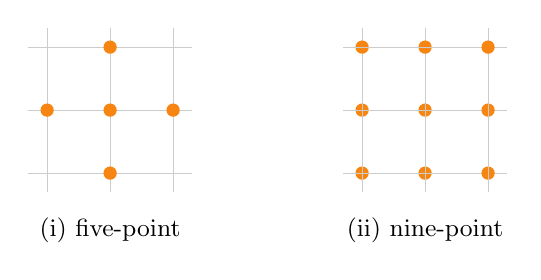
\begin{tikzpicture}[scale=0.8,every node/.style={font=\small}]
\begin{scope}
\foreach \x in {-1,0,1} \foreach \y in {-1,0,1} \draw[gray!40] (\x,-1.3)--(\x,1.3) (-1.3,\y)--(1.3,\y);
\foreach \p in {(0,0),(1,0),(-1,0),(0,1),(0,-1)} \fill[BurntOrange] \p circle (3pt);
\node at (0,-1.9) {(i) five-point};
\end{scope}
\begin{scope}[xshift=5cm]
\foreach \x in {-1,0,1} \foreach \y in {-1,0,1} {\draw[gray!40] (\x,-1.3)--(\x,1.3) (-1.3,\y)--(1.3,\y); \fill[BurntOrange] (\x,\y) circle (3pt);}
\node at (0,-1.9) {(ii) nine-point};
\end{scope}
\end{tikzpicture}

\small Points at level \(n\) used to compute \(U_{l,m}^{n+1}\).
\end{center}

\subsection{Variable coefficients, self-adjoint form}

\[
  \pd ut=\sum_{i=1}^2\pd{}{x_i}\Bigl(a_i(x_1,x_2,t)\pd u{x_i}\Bigr),
  \qquad L=D_1(a_1D_1)+D_2(a_2D_2).
\]
Then
\[
  u_{l,m}^{n+1}=\exp(kL)\,u_{l,m}^n
  =\exp\bigl(kD_1(a_1D_1)\bigr)\exp\bigl(kD_2(a_2D_2)\bigr)u_{l,m}^n,
\]
provided \(D_1(a_1D_1)\) and \(D_2(a_2D_2)\) commute.  Use the
approximations
\[
\begin{gathered}
  D_1(a_1D_1)\approx\frac1{h^2}\delta_{x_1}(a_1\delta_{x_1}),
  \\
  D_2(a_2D_2)\approx\frac1{h^2}\delta_{x_2}(a_2\delta_{x_2}).
\end{gathered}
\]
Applying \(\delta\) twice, with the coefficient evaluated at half
points,
\begin{align*}
  D_1(a_1D_1)U_{l,m}^n
  &\approx\frac1{h^2}\delta_{x_1}\Bigl[a_1\bigl(U_{l+\frac12,m}^n
    -U_{l-\frac12,m}^n\bigr)\Bigr]\\
  &=\frac1{h^2}\Bigl[(a_1)_{l+\frac12,m}\bigl(U_{l+1,m}^n-U_{l,m}^n\bigr)
    -(a_1)_{l-\frac12,m}\bigl(U_{l,m}^n-U_{l-1,m}^n\bigr)\Bigr],
\end{align*}
and similarly for \(D_2(a_2D_2)U^n_{l,m}\) with half points in \(m\).
Expanding to first order in \(k\),
\[
  U_{l,m}^{n+1}
  =\Bigl[1+\frac k{h^2}\Bigl(\delta_{x_1}(a_1\delta_{x_1})
    +\delta_{x_2}(a_2\delta_{x_2})\Bigr)\Bigr]U_{l,m}^n,
\]
that is,
\begin{align*}
  U_{l,m}^{n+1}=U_{l,m}^n+r\Bigl\{
  &(a_1)_{l+\frac12,m}^n\bigl(U_{l+1,m}^n-U_{l,m}^n\bigr)
   -(a_1)_{l-\frac12,m}^n\bigl(U_{l,m}^n-U_{l-1,m}^n\bigr)\\
  +\,&(a_2)_{l,m+\frac12}^n\bigl(U_{l,m+1}^n-U_{l,m}^n\bigr)
   -(a_2)_{l,m-\frac12}^n\bigl(U_{l,m}^n-U_{l,m-1}^n\bigr)\Bigr\}.
\end{align*}
If \(a_1=a_2=1\), this reduces to the five-point scheme
\eqref{eq:five2d}.

\subsection{Stability of the explicit 2D scheme}

For a single harmonic, the harmonic decomposition of the error at
\(t=0\) gives terms of the form \(e^{i\beta x_1}e^{i\gamma x_2}\).  At
\(t=nk\) the solution of the error equation is
\(e^{\alpha t}e^{i\beta x_1}e^{i\gamma x_2}\), so \(e^{\alpha t}\) is
the growth factor of the initial error.  For stability we need
\(|e^{\alpha k}|\le1\) for all \(\beta,\gamma\), since
\((e^{\alpha k})^n\) must stay bounded.

\begin{keybox}
\begin{theorem}[2D explicit scheme]\label{thm:vn2d}
The five-point explicit scheme \eqref{eq:five2d} has amplification
factor
\[
  \xi=1-4r\Bigl(\sin^2\frac{\beta h}2+\sin^2\frac{\gamma h}2\Bigr),
\]
and is stable if and only if \(0<r\le\frac14\).  In \(d\) space
dimensions the condition is \(r\le\frac1{2d}\).
\end{theorem}
\end{keybox}

\begin{proof}
The perturbed solution \(\widetilde U\) satisfies \eqref{eq:five2d}
too, so the error \(z_{l,m}^n=U_{l,m}^n-\widetilde U_{l,m}^n\)
satisfies
\[
  z_{l,m}^{n+1}=(1-4r)z_{l,m}^n
  +r\bigl(z_{l+1,m}^n+z_{l-1,m}^n+z_{l,m+1}^n+z_{l,m-1}^n\bigr).
\]
Let \(z_{l,m}^n=e^{\alpha nk}e^{i\beta lh}e^{i\gamma mh}\).  Substituting
and cancelling \(e^{\alpha nk}e^{i\beta lh}e^{i\gamma mh}\),
\[
  e^{\alpha k}
  =(1-4r)+r\bigl(e^{i\beta h}+e^{-i\beta h}+e^{i\gamma h}+e^{-i\gamma h}\bigr)
  =(1-4r)+2r(\cos\beta h+\cos\gamma h).
\]
With \(\cos\theta=1-2\sin^2\frac\theta2\),
\[
  \xi=(1-4r)+2r\Bigl(2-2\sin^2\frac{\beta h}2-2\sin^2\frac{\gamma h}2\Bigr)
  =\boxed{1-4r\Bigl(\sin^2\frac{\beta h}2+\sin^2\frac{\gamma h}2\Bigr)}.
\]
Stability requires \(|\xi|\le1\).  The right-hand inequality
\(\xi\le1\) holds for \(r>0\).  The left-hand one gives
\[
  -1\le1-4r\Bigl(\sin^2\frac{\beta h}2+\sin^2\frac{\gamma h}2\Bigr)
  \iff
  r\le\frac1{2\bigl(\sin^2\frac{\beta h}2+\sin^2\frac{\gamma h}2\bigr)}.
\]
The bracket can be as large as \(2\), so
\[
  \boxed{0<r\le\tfrac14}
\]
is the condition for stability.  In \(d\) dimensions the bracket is a
sum of \(d\) terms and can be as large as \(d\), giving
\(r\le\frac1{2d}\).
\end{proof}

\begin{remark}[The nine-point scheme]
For scheme (ii), the growth factor factorises:
\[
  \xi=\Bigl(1-4r\sin^2\tfrac{\beta h}2\Bigr)\Bigl(1-4r\sin^2\tfrac{\gamma h}2\Bigr).
\]
Each factor has modulus at most \(1\) when \(0<r\le\frac12\), so the
nine-point scheme is stable for \(0<r\le\frac12\).  It allows twice the
time step of the five-point scheme.
\end{remark}
\end{document}
